%% =====================================================================
%%  M.Tech Project Report  -  Vadithe Sai Kumar Naik (CS25M053)
%%  PDDL-Based Mission Planning for a Fault-Aware Drone Swarm Simulator
%%  Department of Computer Science and Engineering, IIT Madras
%%
%%  Build:  pdflatex main.tex   (run twice so contents and lists update)
%%          or  tectonic main.tex
%%  Files:  figures/iitm_logo.png   pddl/*.pddl  (used in Appendix A)
%% =====================================================================
\documentclass[11pt,a4paper,oneside]{report}

%% ---------- Personal details (edit here) ----------------------------
\newcommand{\thesistitle}{PDDL-Based Mission Planning for a Fault-Aware Drone Swarm Simulator}
\newcommand{\thesistitlebreak}{PDDL-Based Mission Planning for a\\ Fault-Aware Drone Swarm Simulator}
\newcommand{\authorname}{Vadithe Sai Kumar Naik}
\newcommand{\rollno}{CS25M053}
\newcommand{\submitdate}{November 2026}
\newcommand{\advisor}{Dr. N. S. Narayanaswamy}
\newcommand{\coadvisor}{Dr. Jaimandeep Singh}

%% ---------- Packages -------------------------------------------------
\usepackage{iftex}
\ifXeTeX
  \usepackage{newtxtext,newtxmath}
  \setmonofont[Scale=0.95,BoldFont=Inconsolatazi4-Bold.otf]{Inconsolatazi4-Regular.otf}
\else
  \usepackage[T1]{fontenc}
  \usepackage[utf8]{inputenc}
  \usepackage{newtxtext,newtxmath}
  \usepackage[varqu,scaled=0.95]{zi4}
\fi
\usepackage{xstring}
\usepackage[a4paper,top=1in,bottom=1in,left=1.2in,right=1in]{geometry}
\usepackage{setspace}
\setstretch{1.3}
\usepackage{graphicx}
\usepackage{booktabs,tabularx,array,multirow,longtable}
\newcolumntype{Y}{>{\raggedright\arraybackslash}X}
\newcolumntype{P}[1]{>{\raggedright\arraybackslash}p{#1}}
\usepackage{enumitem}
\setlist{itemsep=1pt,topsep=4pt}
\usepackage[table]{xcolor}
\usepackage{amsmath}
\usepackage{listings}
\usepackage{tikz}
\usetikzlibrary{arrows.meta,positioning,shapes.geometric,shapes.misc,fit,calc,backgrounds,decorations.pathreplacing}
\usepackage{pgfplots}
\pgfplotsset{compat=1.17}
\usepackage[font=small,labelfont=bf,labelsep=colon]{caption}
\captionsetup[table]{justification=raggedright,singlelinecheck=false,skip=6pt}
\captionsetup[figure]{format=hang,skip=6pt}
\usepackage{titlesec}
\usepackage{titletoc}
\usepackage{float}
\usepackage{xurl}
\usepackage[hidelinks]{hyperref}
\hypersetup{
  pdftitle={\thesistitle},
  pdfauthor={\authorname},
  pdfsubject={M.Tech thesis, IIT Madras}
}

%% ---------- Colours --------------------------------------------------
\definecolor{navy}{HTML}{0F2240}
\definecolor{amber}{HTML}{F0A30A}
\definecolor{codebg}{HTML}{F5F5F5}
\definecolor{coderule}{HTML}{C8C8C8}
\definecolor{kwblue}{HTML}{1F5FBF}
\definecolor{cmtgray}{HTML}{7A7A7A}
\definecolor{okgreen}{HTML}{2E7D32}
\definecolor{warnred}{HTML}{C62828}
\definecolor{softblue}{HTML}{E8EEF7}
\definecolor{softamber}{HTML}{FDF1D8}

%% ---------- Chapter and section headings ----------------------------
\titleformat{\chapter}[display]
  {\centering\bfseries}
  {\LARGE\chaptertitlename\ \thechapter}
  {1.6em}
  {\huge}
\titlespacing*{\chapter}{0pt}{10pt}{28pt}
\titleformat{name=\chapter,numberless}[block]
  {\centering\bfseries\huge}{}{0pt}{}
\titlespacing*{name=\chapter,numberless}{0pt}{10pt}{24pt}
\titleformat{\section}{\bfseries\Large}{\thesection}{0.6em}{}
\titleformat{\subsection}{\bfseries\large}{\thesubsection}{0.6em}{}
\titleformat{\paragraph}[runin]{\bfseries}{}{0pt}{}[.]
\titlespacing*{\section}{0pt}{20pt}{10pt}
\titlespacing*{\subsection}{0pt}{14pt}{6pt}
\setcounter{secnumdepth}{3}
\setcounter{tocdepth}{2}

%% ---------- Contents, list of tables, list of figures ---------------
\renewcommand{\contentsname}{Contents}
\renewcommand{\listtablename}{List of Tables}
\renewcommand{\listfigurename}{List of Figures}
\titlecontents{chapter}[0pt]
  {\addvspace{1.1em}\bfseries}
  {\makebox[7.2em][l]{\IfInteger{\thecontentslabel}{CHAPTER}{APPENDIX} \thecontentslabel}\MakeUppercase}
  {\MakeUppercase}
  {\hfill\contentspage}
  [\addvspace{0.4em}]
\titlecontents{section}[4.2em]
  {\small}
  {\contentslabel{4.2em}}
  {}
  {\titlerule*[0.7pc]{.}\contentspage}
\titlecontents{subsection}[4.2em]
  {\small}
  {\contentslabel{4.2em}}
  {}
  {\titlerule*[0.7pc]{.}\contentspage}
\titlecontents{figure}[4.2em]
  {\small}
  {\contentslabel{2.8em}}
  {}
  {\titlerule*[0.7pc]{.}\contentspage}
\titlecontents{table}[4.2em]
  {\small}
  {\contentslabel{2.8em}}
  {}
  {\titlerule*[0.7pc]{.}\contentspage}
% Front-matter entries in the contents (bold, upper case, no dots)
\newcommand{\addfront}[1]{%
  \addtocontents{toc}{\protect\noindent\protect\rule{0pt}{2.1em}\protect\textbf{#1}\protect\hfill\protect\textbf{\thepage}\protect\par}}

%% ---------- Code listings (PDDL) -------------------------------------
\lstdefinelanguage{PDDL}{
  morekeywords=[1]{define,domain,problem,and,or,not,forall,exists,when,imply,
    increase,decrease,assign,either},
  morekeywords=[2]{:requirements,:types,:predicates,:functions,:action,
    :parameters,:precondition,:effect,:objects,:init,:goal,:domain,:strips,
    :typing,:numeric-fluents,:negative-preconditions,:conditional-effects,
    :equality,:disjunctive-preconditions,:universal-preconditions},
  sensitive=false,
  morecomment=[l]{;},
  alsoletter={:-},
}
\lstset{
  language=PDDL,
  basicstyle=\ttfamily\footnotesize\setstretch{1.0},
  keywordstyle=[1]\color{kwblue}\bfseries,
  keywordstyle=[2]\color{kwblue},
  commentstyle=\color{cmtgray}\itshape,
  backgroundcolor=\color{codebg},
  frame=single,
  rulecolor=\color{coderule},
  framesep=4pt,
  xleftmargin=6pt,xrightmargin=6pt,
  aboveskip=8pt,belowskip=8pt,
  breaklines=true,
  breakatwhitespace=true,
  columns=fullflexible,
  keepspaces=true,
  showstringspaces=false,
  tabsize=4,
}
\lstdefinestyle{plain}{language={},keywordstyle=,commentstyle=}
\lstdefinestyle{appendix}{basicstyle=\ttfamily\scriptsize\setstretch{1.0},
  numbers=left,numberstyle=\tiny\color{cmtgray},numbersep=6pt,xleftmargin=18pt}

\newcommand{\code}[1]{\texttt{#1}}
\newcommand{\recordlabel}[1]{\par\smallskip\noindent\hspace*{1.2em}\textit{#1}\par}

%% ---------- Reusable TikZ styles -------------------------------------
\tikzset{
  drone/.style={circle,fill=navy,minimum size=7pt,inner sep=0pt},
  leader/.style={circle,fill=amber,minimum size=9pt,inner sep=0pt},
  link/.style={navy,line width=0.7pt},
  box/.style={draw=navy,line width=0.8pt,rounded corners=3pt,fill=softblue,
              align=center,font=\small,inner sep=5pt,minimum height=2.2em},
  abox/.style={box,fill=softamber,draw=amber!80!black},
  gbox/.style={box,fill=white},
  arr/.style={-{Stealth[length=5pt]},line width=0.8pt,navy},
  darr/.style={arr,dashed},
}

\begin{document}

%% =====================================================================
%%  COVER PAGE
%% =====================================================================
\begin{titlepage}
\thispagestyle{empty}
\begin{minipage}[c]{0.36\textwidth}
  
\includegraphics[width=0.62\linewidth]{figures/iitm_logo.png}
\end{minipage}%
\begin{minipage}[c]{0.64\textwidth}
  \setstretch{1.05}\small
  DEPARTMENT OF COMPUTER SCIENCE AND\\
  ENGINEERING\\
  INDIAN INSTITUTE OF TECHNOLOGY MADRAS\\
  CHENNAI -- 600036
\end{minipage}

\vspace{0.6cm}
\noindent\rule{\textwidth}{2pt}

\vspace{2.2cm}
\begin{center}
  {\setstretch{1.2}\LARGE\bfseries \thesistitlebreak\par}

  \vspace{1.6cm}
  % ---- Emblem: a V-formation swarm flying a planned route ----
  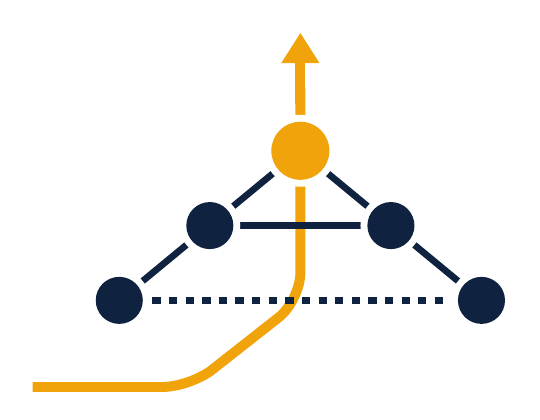
\begin{tikzpicture}[scale=1.0]
    \draw[amber,line width=3.6pt,rounded corners=10pt]
         (-3.4,-2.6)--(-1.4,-2.6)--(0,-1.5)--(0,1.2);
    \draw[amber,line width=3.6pt,-{Triangle[length=11pt,width=13pt]}] (0,1.0)--(0,1.9);
    \coordinate (L)  at (0,0.4);
    \coordinate (A1) at (-1.15,-0.55);
    \coordinate (A2) at (-2.3,-1.5);
    \coordinate (B1) at (1.15,-0.55);
    \coordinate (B2) at (2.3,-1.5);
    \draw[navy,line width=2.4pt] (A2)--(A1)--(L)--(B1)--(B2);
    \draw[navy,line width=2.4pt] (A1)--(B1);
    \draw[navy,line width=2.4pt,dashed] (A2)--(B2);
    \foreach \p in {A1,A2,B1,B2} {\fill[white] (\p) circle (11pt); \fill[navy] (\p) circle (8.5pt);}
    \fill[white] (L) circle (13pt); \fill[amber] (L) circle (10.5pt);
  \end{tikzpicture}

  \vspace{1.8cm}
  {\itshape A Thesis\par}
  \vspace{0.25cm}
  {\itshape Submitted by\par}
  \vspace{0.3cm}
  {\Large\bfseries \authorname\par}
  \vspace{1.0cm}
  {\itshape For the award of the degree\par}
  \vspace{0.25cm}
  {\itshape Of\par}
  \vspace{0.25cm}
  {\bfseries MASTER OF TECHNOLOGY\par}
  \vspace{0.2cm}
  \submitdate
\end{center}
\end{titlepage}

%% =====================================================================
%%  THESIS CERTIFICATE
%% =====================================================================
\thispagestyle{empty}
\begin{center}
  {\LARGE\bfseries Thesis Certificate\par}
\end{center}
\vspace{0.8cm}
\noindent This is to certify that the thesis entitled \textbf{\thesistitle}, submitted by
\textbf{\authorname\ (\rollno)} to the Indian Institute of Technology Madras in partial
fulfilment of the requirements for the degree of \textbf{Master of Technology}, is a bona fide
record of the work carried out under the guidance of \textbf{\advisor}, Project Advisor, and
\textbf{\coadvisor}, Project Co-Advisor.

\noindent The contents of this thesis, in full or in part, have not been submitted to any other
institute or university for the award of a degree or diploma.

\vspace{2.2cm}
\noindent
\begin{minipage}[t]{0.5\textwidth}
  \setstretch{1.15}
  Chennai 600036\\
  Date: \submitdate
\end{minipage}%
\begin{minipage}[t]{0.5\textwidth}
  \raggedleft\setstretch{1.15}
  \textbf{\authorname}\\
  \rollno
\end{minipage}

\vspace{2.6cm}
\begin{flushright}
  \setstretch{1.15}
  \textbf{\advisor}\\
  Project Advisor, Professor\\
  Department of Computer Science and Engineering\\
  Indian Institute of Technology Madras
\end{flushright}

\vspace{1.8cm}
\begin{flushright}
  \setstretch{1.15}
  \textbf{\coadvisor}\\
  Project Co-Advisor\\
  Department of Computer Science and Engineering\\
  Indian Institute of Technology Madras
\end{flushright}

\vfill
\noindent{\small \textcopyright\ 2026 Indian Institute of Technology Madras}
\clearpage

%% =====================================================================
%%  FRONT MATTER
%% =====================================================================
\pagenumbering{roman}
\pagestyle{plain}

\addtocontents{toc}{\protect\noindent\protect\hfill\protect\textbf{Page}\protect\par}
\addtocontents{lot}{\protect\noindent\protect\makebox[4.2em][l]{\protect\textbf{Table}}\protect\hfill\protect\textbf{Caption}\protect\hfill\protect\textbf{Page}\protect\par\protect\vspace{0.6em}}
\addtocontents{lof}{\protect\noindent\protect\makebox[4.2em][l]{\protect\textbf{Figure}}\protect\hfill\protect\textbf{Caption}\protect\hfill\protect\textbf{Page}\protect\par\protect\vspace{0.6em}}
\chapter*{Acknowledgements}
\addfront{ACKNOWLEDGEMENTS}
I express my sincere gratitude to \textbf{\advisor}, Project Advisor, and
\textbf{\coadvisor}, Project Co-Advisor, for their guidance, feedback and encouragement
throughout this project. Their insistence on clear models, careful testing and honest
reporting of limitations shaped the way the planning work in this thesis was designed and
verified.

I thank the Department of Computer Science and Engineering, Indian Institute of Technology
Madras, for the facilities and academic environment that supported this work. I also thank my
project teammates, who built and maintained the other parts of the drone swarm simulator, for
many useful discussions on how the planner should connect to the ground station and to the
flight software.

Finally, I thank my family and friends for their constant support during the project and the
preparation of this report. The responsibility for the analysis and conclusions presented here
rests with the author.

\chapter*{Abstract}
\addfront{ABSTRACT}
\noindent\textbf{Keywords:} automated planning; PDDL; numeric planning; ENHSP; drone swarm;
formation flight; fault handling; battery management.

\medskip
A drone swarm mission is more than a route. Before a drone may take off, join a formation or
continue a leg, its battery must cover the next move, its GPS and radio links must work, its
health must be acceptable and its neighbours in the formation must be in place. This thesis
describes the planning layer of a software-in-the-loop drone swarm simulator, in which these
rules are written in the Planning Domain Definition Language (PDDL) and solved by the
Expressive Numeric Heuristic Search Planner (ENHSP). The complete PDDL layer is the author's
contribution to the project.

Ten mission plans were developed, each as a domain file and a problem template: point-to-point
travel, forest area search, V formation, two-dimensional grid formation, three-dimensional
(cube) grid formation, parabola formation, figure-eight train formation, star drone show,
planetary orbit show and road inspection. Every plan shares one vocabulary of drone states,
health flags, failure states and numeric fluents for battery, energy, altitude and health. A
plan service retargets each template onto the points the operator picks on the map, expands it
to the number of selected drones and passes it to ENHSP. Only the leader corridor is usually
planned symbolically; the other drones' routes are then derived geometrically from their
formation slots.

Inter-drone communication is modelled in two layers. In PDDL, each formation declares which
drones are neighbours and every formation action checks a per-drone \code{neighbor-comm-ok}
flag; the parabola plan goes further and requires each directed link to be established within
a communication range. At run time the ground station talks to each drone over a JSON-over-UDP
protocol with heartbeats, and formation keeping for trains and shows runs on board each drone
against a shared, time-stamped pace. Four fault types are modelled in the domains -- GPS loss,
communication loss, neighbour-link loss and health failure -- together with ground-controller
responses such as return, hover and sacrifice. Battery health is handled both as a planning
resource (energy per metre, climb and leg energy, a 30-unit reserve) and at run time through
low (20\,\%) and critical (5\,\%) thresholds that pause the swarm and ask the operator to decide.

The plans were exercised through the real planning pipeline. On the run logs, the forest search
solved 69 of 69 requests and point-to-point travel 76 of 83, with all failures traced to
infeasible map inputs. The cube formation solves 64 drones in 50\,s and the figure-eight train
solves up to its computed capacity of 27 drones while correctly rejecting 28. The report also
records the modelling defects that were found and fixed, and the limits of the present
approach.

\tableofcontents
\addtocontents{toc}{\protect\vspace{-1.2em}}
\clearpage
\addfront{LIST OF TABLES}
\listoftables
\clearpage
\addfront{LIST OF FIGURES}
\listoffigures

\chapter*{Abbreviations}
\addfront{ABBREVIATIONS}
\begin{center}
\begin{tabular}{@{}p{0.22\textwidth}p{0.68\textwidth}@{}}
\toprule
\textbf{Abbreviation} & \textbf{Meaning} \\
\midrule
PDDL   & Planning Domain Definition Language \\
ENHSP  & Expressive Numeric Heuristic Search Planner \\
GCS    & Ground Control Station \\
GUI    & Graphical User Interface \\
UAV    & Unmanned Aerial Vehicle \\
SYSID  & MAVLink system identifier of a drone \\
MAVLink& Micro Air Vehicle Link, a lightweight drone messaging protocol \\
SITL   & Software in the Loop \\
UDP    & User Datagram Protocol \\
JSON   & JavaScript Object Notation \\
OSRM   & Open Source Routing Machine \\
AIBR   & Additive Interval Based Relaxation (ENHSP preprocessing) \\
RTL    & Return to Launch \\
\bottomrule
\end{tabular}
\end{center}

\clearpage
\pagenumbering{arabic}

%% =====================================================================
%%  CHAPTER 1  INTRODUCTION
%% =====================================================================
\chapter{Introduction}

\section{Background and Motivation}
Small unmanned aerial vehicles are now used for search, inspection, mapping and public light
shows. Many of these tasks are done better by a group of drones than by one drone. A group,
however, needs coordination. Each drone must know when to take off, which place in the
formation it must hold, which other drones it must stay in contact with, and what to do when
something goes wrong. Writing these rules directly in flight code makes them hard to read, hard
to check and hard to change.

Automated planning offers a cleaner way. In planning, the rules of the world are written once as
a \emph{domain}: a set of actions, each with the conditions under which it may be applied and the
changes it causes. A particular mission is written as a \emph{problem}: the drones, the places,
the starting state and the goal. A general-purpose planner then searches for a sequence of
actions that reaches the goal while respecting every rule. PDDL is the standard language for
writing such domains and problems~\cite{mcdermott1998pddl,fox2003pddl21}.

This project is part of a larger drone swarm simulator built in the department. The simulator
runs each drone as an independent thread (and, optionally, real flight firmware under
emulation), and offers a ground station GUI with a map, telemetry and fault injection. The work
reported here is the planning layer of that simulator: the PDDL models for every mission type,
and their link to the rest of the system.

\section{Problem Statement and Objectives}
The central problem is to express swarm missions -- including formations, communication
requirements, battery limits and failures -- in PDDL in a way that a numeric planner can solve
quickly for realistic swarm sizes, and whose plans can be turned into flyable routes. The work
had the following objectives:
\begin{enumerate}
  \item Design a common PDDL vocabulary for drone state, health, communication, battery and
        failure that every mission plan can share.
  \item Build domain and problem files for a range of missions: travel, area search, rigid
        formations (V, grid, cube, parabola), path-following trains (figure-eight), shape-changing
        shows (star, planets) and road inspection.
  \item Model drone-to-drone communication, so that a formation can only form and fly while the
        required links are up.
  \item Model faults (GPS, communication, neighbour link, health) and battery health, together
        with the ground controller's responses.
  \item Integrate the plans with the simulator, so that a plan is retargeted to the operator's map
        inputs, solved by ENHSP and executed by the drones, and verify the results.
\end{enumerate}

\section{Scope and Contributions}
The author's contribution is the complete PDDL layer of the simulator. This thesis contributes:
\begin{itemize}
  \item ten mission plans (Table~\ref{tab:inventory}), about 6\,700 lines of PDDL in total,
        written on one shared vocabulary of predicates and numeric fluents;
  \item a set of modelling patterns that keep formation problems tractable for large swarms:
        planning only the leader corridor, descriptive neighbour relations with per-drone
        communication flags, and propositional rather than numeric gates for ordered launches;
  \item a two-level model of communication: symbolic neighbour links in PDDL, including an
        explicit range-checked link model in the parabola plan, and the run-time protocol used
        by the ground station and the drones;
  \item a fault and battery model covering four failure types, ground-controller responses and
        energy accounting for travel, climb, cruise and hover;
  \item verification of every plan through the real planning pipeline, including scalability
        measurements and a record of the modelling defects found and fixed.
\end{itemize}

The GUI, the drone threads, the firmware emulation and the map services were built by the
project team. They are described here only as far as needed to explain how a PDDL plan
becomes a flight. Physical flight tests are outside the scope of this report; all results
are from the simulator.

\section{Organisation of the Report}
Chapter~\ref{ch:background} reviews automated planning, PDDL, numeric planning and related work
on multi-drone missions. Chapter~\ref{ch:arch} explains the simulator architecture and the
planning pipeline. Chapter~\ref{ch:model} presents the common PDDL vocabulary and design
patterns. Chapter~\ref{ch:plans} describes all ten mission plans. Chapter~\ref{ch:comm}
explains how drones communicate, both in the model and at run time. Chapter~\ref{ch:faults}
covers fault modelling and battery health. Chapter~\ref{ch:results} reports the verification
results and the defects found. Chapter~\ref{ch:discussion} discusses limitations, and
Chapter~\ref{ch:conclusion} concludes with future work. Appendix~\ref{app:pddl} lists complete
PDDL sources for two of the plans.

%% =====================================================================
%%  CHAPTER 2  BACKGROUND AND LITERATURE REVIEW
%% =====================================================================
\chapter{Background and Literature Review}\label{ch:background}

\section{Automated Planning}
Classical planning studies how an agent can reach a goal from a known initial state by applying
actions with known effects~\cite{ghallab2004automated}. A planning task is described by a set of
state variables, a set of actions and a goal. Each action has a \emph{precondition} that must
hold before it is applied and an \emph{effect} that changes the state. A \emph{plan} is a sequence
of actions that, applied in order from the initial state, ends in a state that satisfies the
goal. Heuristic search planners find such plans by estimating, for each state, how far it is
from the goal and expanding the most promising states first.

\section{The Planning Domain Definition Language}
PDDL was introduced to give planning competitions a common input
language~\cite{mcdermott1998pddl}. A PDDL model is split into two files:
\begin{itemize}
  \item the \textbf{domain} defines object types, \emph{predicates} (true/false facts such as
        \code{(gps-ok ?d)}), \emph{functions} (numeric values such as \code{(battery ?d)}) and
        \emph{actions};
  \item the \textbf{problem} names the concrete objects, gives the initial facts and values, and
        states the goal.
\end{itemize}
PDDL\,2.1 added numeric fluents, so that actions can test and change numbers, for example
\code{(> (battery ?d) (energy-required ?from ?to))} as a precondition and
\code{(decrease (battery ?d) ...)} as an effect~\cite{fox2003pddl21}. Later requirements such as
\code{:conditional-effects}, \code{:universal-preconditions} and \code{:negative-preconditions}
allow an action to say ``for every wing drone, \ldots'' or ``only if this drone is \emph{not}
already in formation''. All of these features are used in this work.

\section{Numeric Planning with ENHSP}
ENHSP is a heuristic search planner for PDDL\,2.1 problems with numeric
fluents~\cite{scala2016interval,scala2020subgoaling}. It grounds the domain into concrete actions,
runs a relaxation-based preprocessing step (AIBR) that also detects some unsolvable problems
early, and then searches with numeric heuristics. Two properties of ENHSP mattered in this
project. First, its heuristics estimate progress well for conditions that compare a fluent with
a constant, but poorly for conditions that compare two fluents with each other. Second, its
grounding step can use a large amount of memory for domains with many drones and quantified
conditions; a ``naive'' grounder option (\code{-gro naive}) helps for formation domains. Both
points shaped the models in Chapter~\ref{ch:model}.

\section{Multi-Drone Missions and Formations}
Aerial swarm research covers formation control, task allocation and collective
behaviour~\cite{chung2018survey,brambilla2013swarm}. Formation flight is often treated with a
leader--follower scheme, in which one drone follows the planned path and the others hold an
offset from it. Early work on flocking showed that simple local rules with near neighbours are
enough for coherent group motion~\cite{reynolds1987flocks}. This project borrows both ideas: the
planner reasons about a leader corridor, and each drone is required to stay in contact only with
its immediate neighbours. For curved paths, shortest paths with a bounded turning radius were
characterised by Dubins~\cite{dubins1957curves}, and such paths are used to join the figure-eight
pattern smoothly.

\section{Fault-Aware Planning for UAVs}
Real drones lose GPS, lose radio contact and run out of battery. A plan that ignores these events
is not safe to fly. In planning, faults are commonly handled either by monitoring execution and
replanning, or by including recovery actions in the domain. This work follows the second idea in
a light form: each domain includes detection actions that turn a failed health flag into a failure
state and a controller notification, and the point-to-point domain adds explicit controller
orders (return, hover, sacrifice). Battery is treated as a numeric resource, so that the planner
itself refuses any move the drone cannot afford.

\section{Position of This Work}
The contribution is not a new planning algorithm. It is a family of carefully engineered PDDL
models for drone swarm missions, connected to a working simulator, together with an honest record
of what the models express, how they scale and where they stop. The models are written to be
read by people as well as solved by a planner, so that a supervisor or teammate can check every
safety rule directly in the PDDL.

%% =====================================================================
%%  CHAPTER 3  SYSTEM ARCHITECTURE
%% =====================================================================
\chapter{System Architecture and Planning Pipeline}\label{ch:arch}

\section{Simulator Overview}
The simulator has four main parts. The \textbf{ground station GUI} (PySide6) shows the map,
telemetry, the mission planner panel and fault injection controls. The \textbf{plan service}
prepares PDDL problems and calls the planner. The \textbf{planner} is ENHSP, run as a Java
process. The \textbf{drones} are independent threads, each with its own state, command inbox and
telemetry output; a drone can also be backed by real flight firmware running under Renode
emulation. Table~\ref{tab:components} summarises the roles.

\begin{table}[H]
\caption{Components of the simulator and their role in planning}\label{tab:components}
\small
\begin{tabularx}{\textwidth}{@{}P{0.27\textwidth}Y@{}}
\toprule
\textbf{Component} & \textbf{Responsibility} \\
\midrule
Mission planner panel (GUI) & Choose a named plan, pick source, destination, area or pattern
points on the map, set laps and show speed. \\
Plan service (\code{services/plan\_service.py}) & Select the plan folder, retarget the template
to the picked points, expand it to $N$ drones, call ENHSP, check the returned action order and
build per-drone routes. \\
Problem tools (\code{engine/pddl\_problem.py} and per-plan modules) & Rewrite coordinates,
distances and energy facts; clone template drones; build neighbour chains and geometry. \\
ENHSP (\code{engine/pddl\_planner.py}) & Ground and solve the problem; return the plan text,
which is parsed into ordered steps. \\
Thread backend and GCS (\code{services/thread\_backend.py}, \code{engine/gcs.py}) & Send
missions and commands to each drone, receive telemetry and heartbeats, keep formation pace and
raise low-battery, GPS-loss and drone-lost events. \\
Drone thread (\code{engine/drone\_thread.py}) & Integrate motion and battery, monitor health
and communication, fly the uploaded route. \\
\bottomrule
\end{tabularx}
\end{table}

\section{From Map Clicks to Flying Drones}
Figure~\ref{fig:pipeline} shows the planning pipeline. Every plan folder under \code{plans/}
holds one \code{domain.pddl} and one problem template. The template is written for a small,
fixed example (for example one leader and two wings). When the operator picks points on the map,
the plan service \emph{retargets} the template: it replaces the coordinates, recomputes each
edge's distance and \code{energy-required} at that edge's own energy-per-metre rate, and, if a
restricted area was marked, inserts detour locations. It then \emph{expands} the template to the
number of selected drones by cloning the template drone's facts line by line and rebuilding the
neighbour relations. The resulting problem is passed to ENHSP. The returned plan is checked
against the order of actions the plan kind expects, and the leader's corridor is extracted.
Finally, member routes are derived from the corridor and the slot offsets, and the routes are
uploaded to the drones as whole missions.

\begin{figure}[H]
\centering
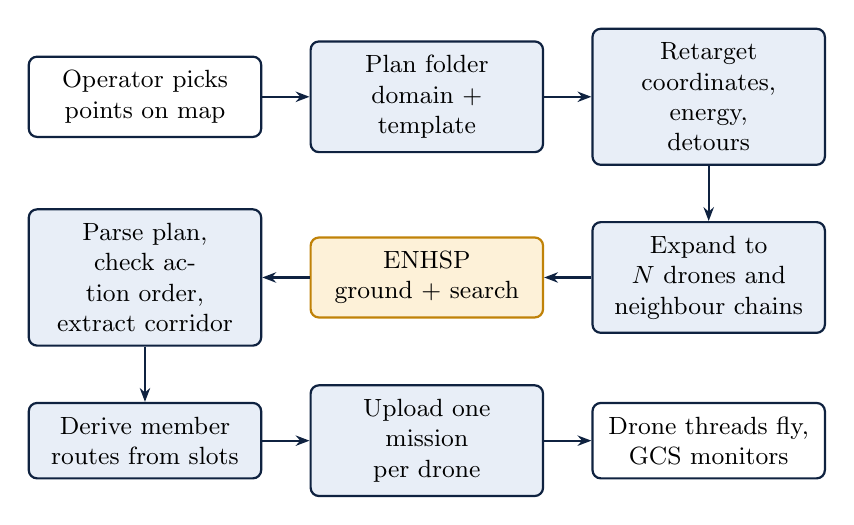
\begin{tikzpicture}[node distance=7mm and 6mm]
  \node[gbox,text width=2.6cm] (gui) {Operator picks\\points on map};
  \node[box,right=of gui,text width=2.6cm] (tpl) {Plan folder\\domain + template};
  \node[box,right=of tpl,text width=2.6cm] (ret) {Retarget\\coordinates, energy,\\detours};
  \node[box,below=of ret,text width=2.6cm] (exp) {Expand to\\$N$ drones and\\neighbour chains};
  \node[abox,left=of exp,text width=2.6cm] (enhsp) {ENHSP\\ground + search};
  \node[box,left=of enhsp,text width=2.6cm] (chk) {Parse plan,\\check action order,\\extract corridor};
  \node[box,below=of chk,text width=2.6cm] (der) {Derive member\\routes from slots};
  \node[box,right=of der,text width=2.6cm] (up) {Upload one mission\\per drone};
  \node[gbox,right=of up,text width=2.6cm] (fly) {Drone threads fly,\\GCS monitors};
  \draw[arr] (gui)--(tpl);
  \draw[arr] (tpl)--(ret);
  \draw[arr] (ret)--(exp);
  \draw[arr] (exp)--(enhsp);
  \draw[arr] (enhsp)--(chk);
  \draw[arr] (chk)--(der);
  \draw[arr] (der)--(up);
  \draw[arr] (up)--(fly);
\end{tikzpicture}
\caption{The planning pipeline, from the operator's map input to the drones' flight.}
\label{fig:pipeline}
\end{figure}

\section{Plan Kinds and Folders}
The plan service decides how to treat a plan from the \emph{domain name} written inside
\code{domain.pddl}, not from the folder name. This lets a folder be renamed freely and makes the
domain file the single source of truth. Table~\ref{tab:inventory} lists all ten plans.

\begin{table}[H]
\caption{Inventory of the ten mission plans}\label{tab:inventory}
\small
\begin{tabularx}{\textwidth}{@{}l>{\ttfamily\footnotesize}P{0.36\textwidth}lY@{}}
\toprule
\textbf{Folder} & \textbf{\normalfont\small Domain name} & \textbf{Kind} & \textbf{Drones} \\
\midrule
\code{travell}           & swarm-drone-mission               & point\_to\_point    & 1 or more \\
\code{Search}            & forest-drone-search               & area\_coverage      & $\geq 2$ \\
\code{vformation}        & v-formation-drone-mission         & formation           & odd, $\geq 3$ \\
\code{gridformation}     & grid-formation-drone-mission      & grid\_formation     & $\geq 4$ \\
\code{3dgridformation}   & cube-grid-formation-drone-mission & cube\_formation     & $\geq 8$ \\
\code{parabolaformation} & parabola-formation-drone-mission  & parabola\_formation & exactly 3 \\
\code{figure8formation}  & figure8-formation-drone-mission   & figure8\_formation  & 2 to capacity \\
\code{starformation}     & star-formation-drone-mission      & star\_formation     & 6 to 40 \\
\code{planets}           & planets-formation-drone-mission   & planets\_formation  & 2 to 8 \\
\code{Inspect}           & road-inspection-drone-mission     & road\_inspection    & 1 \\
\bottomrule
\end{tabularx}
\end{table}

\section{Run Records}
Every planning request writes a time-stamped folder under \code{plans/<name>/runs/} containing
the exact problem that was solved and the full ENHSP output. These records made it possible to
trace every unsolvable request back to its input, and they are the source of the statistics in
Chapter~\ref{ch:results}.

%% =====================================================================
%%  CHAPTER 4  PDDL MODELLING APPROACH
%% =====================================================================
\chapter{PDDL Modelling Approach}\label{ch:model}

\section{A Shared Vocabulary}
All ten domains use the same core vocabulary, so that a reader who understands one plan can read
any other. The domains declare the types \code{drone}, \code{location} and \code{controller}
(plus plan-specific types such as \code{forest-area} or \code{layer}). Table~\ref{tab:vocab}
lists the shared predicates and functions.

\begin{table}[H]
\caption{Shared predicates and numeric functions used across the domains}\label{tab:vocab}
\small
\begin{tabularx}{\textwidth}{@{}>{\ttfamily\footnotesize}P{0.38\textwidth}Y@{}}
\toprule
\textbf{\normalfont\small Symbol} & \textbf{Meaning} \\
\midrule
\multicolumn{2}{@{}l}{\textit{Position and flight state}} \\
(at ?d ?l), (formation-at ?l) & Where a drone, or the whole formation, is. \\
(landed ?d), (airborne ?d), (flying ?d) & Flight phase of a drone. \\
(at-cruise-altitude ?d) & Drone has climbed to its own target altitude. \\
(connected ?a ?b), (safe-route ?a ?b) & A leg exists and avoids restricted areas. \\
\midrule
\multicolumn{2}{@{}l}{\textit{Health and communication}} \\
(gps-ok ?d), (communication-ok ?d) & GPS fix and link to the ground controller are working. \\
(drone-healthy ?d) & Airframe passes its health check. \\
(neighbor-comm-ok ?d) & Drone-to-drone links to its formation neighbours are working. \\
(gps-lost ?d), (communication-lost ?d), (health-failure ?d) & Failure states set by
detection actions. \\
(controller-notified ?d) & Ground controller has been told of a failure. \\
\midrule
\multicolumn{2}{@{}l}{\textit{Numeric fluents}} \\
(battery ?d), (max-battery ?d) & Current and full battery, in model units (100 = full). \\
(minimum-return-battery ?d) & Reserve kept for a safe return (30 in the templates). \\
(energy-required ?a ?b), (distance ?a ?b) & Cost and length of a leg. \\
(climb-energy ?d), (cruise-leg-energy ?d) & Energy for the climb and for one follower leg. \\
(health ?d), (minimum-health ?d) & Health score (100) and its limit (40). \\
(altitude ?d), (hover-altitude ?d), (target-altitude ?d) & Current, hover (2\,m) and cruise
altitude. \\
(slot-along-offset ?d), (slot-cross-offset ?d) & Formation slot relative to the leader, in
metres. \\
\bottomrule
\end{tabularx}
\end{table}

\section{The Common Mission Life Cycle}
Every formation plan follows the same life cycle (Figure~\ref{fig:lifecycle}). A drone first
passes a \code{pre-flight-check}, which needs it to be landed at the source with GPS, radio and
health in order and a battery above its return reserve. It then takes off to hover altitude and
climbs to its own cruise altitude, paying \code{climb-energy}. Once airborne, it takes its slot
in the formation. An \code{establish-...-formation} action fires only when every member is in
its slot, at altitude and in contact with its neighbours. The leader then flies the corridor one
leg at a time with \code{formation-cruise}; after each leg the formation is marked ``open'' and
a close-up action (\code{close-up-wings}, \code{close-up-grid}, \code{hold-parabola-shape},
\code{follow-leader}) must bring every member back into its slot before the next leg. The
mission completes when the closed formation is at the destination.

\begin{figure}[H]
\centering
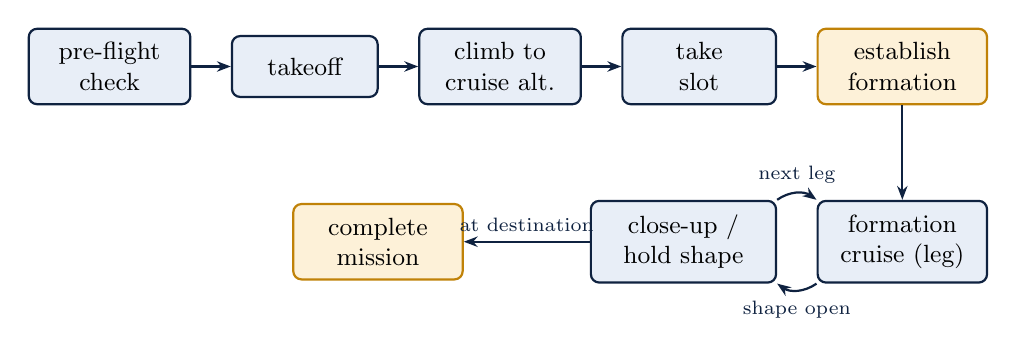
\begin{tikzpicture}[node distance=5mm and 5mm, every node/.style={font=\footnotesize}]
  \node[box,text width=1.7cm] (pf) {pre-flight\\check};
  \node[box,right=of pf,text width=1.5cm] (to) {takeoff};
  \node[box,right=of to,text width=1.7cm] (cl) {climb to\\cruise alt.};
  \node[box,right=of cl,text width=1.6cm] (sl) {take\\slot};
  \node[abox,right=of sl,text width=1.8cm] (es) {establish\\formation};
  \node[box,below=12mm of es,text width=1.8cm] (cr) {formation\\cruise (leg)};
  \node[box,left=of cr,text width=2.0cm] (cu) {close-up /\\hold shape};
  \node[abox,left=16mm of cu,text width=1.8cm] (cm) {complete\\mission};
  \draw[arr] (pf)--(to); \draw[arr] (to)--(cl); \draw[arr] (cl)--(sl); \draw[arr] (sl)--(es);
  \draw[arr] (es)--(cr);
  \draw[arr] (cr.south west) to[bend left=35] node[below,font=\scriptsize]{shape open} (cu.south east);
  \draw[arr] (cu.north east) to[bend left=35] node[above,font=\scriptsize]{next leg} (cr.north west);
  \draw[arr] (cu)--node[above,font=\scriptsize]{at destination}(cm);
\end{tikzpicture}
\caption{The life cycle shared by the formation plans. Each box is one PDDL action (or one
action per drone).}
\label{fig:lifecycle}
\end{figure}

The take-off step itself is short but illustrates the style used throughout:

\begin{lstlisting}
(:action takeoff
    :parameters (?d - drone ?l - location)
    :precondition (and (at ?d ?l) (source ?l) (landed ?d)
                       (preflight-done ?d)
                       (gps-ok ?d) (communication-ok ?d) (drone-healthy ?d))
    :effect (and (not (landed ?d)) (airborne ?d) (flying ?d)
                 (assign (altitude ?d) (hover-altitude ?d))))
\end{lstlisting}

\section{Design Patterns for Tractable Swarm Models}
Swarm problems grow quickly with the number of drones. Four patterns kept the models small
enough for ENHSP to solve within seconds.

\paragraph{Plan the leader, derive the rest}
For rigid formations the planner reasons about the leader's corridor only. Members are moved
together by one close-up action with a universally quantified, conditional effect, instead of
being routed one by one. Their geographic routes are computed afterwards by offsetting the
corridor by the slot offsets. This keeps the number of ground actions close to linear in $N$.

\paragraph{Descriptive neighbours, per-drone flags}
Each formation records which drones are neighbours (\code{wing-neighbor}, \code{grid-neighbor},
\code{cube-neighbor}, \code{train-neighbor}, \code{orbit-neighbor}). In most plans these pairwise
facts are descriptive only: the actions test the per-drone flag \code{neighbor-comm-ok} instead.
A check over all drones is then $O(N)$ rather than $O(N^2)$, which matters most for the cube,
where a full $4\times4\times4$ block declares 420 undirected links.

\paragraph{Propositional gates instead of numeric comparisons}
The cube's layer-by-layer launch was first written with a numeric counter, gating take-off on
\code{(<= (slot-layer ?d) (layers-cleared))}. ENHSP's heuristic estimates almost no progress for
a comparison between two fluents, so a 25-drone, 3-layer block did not solve in 90\,s. The
gate was rewritten with \code{layer} objects chained by \code{(layer-below ?lo ?hi)} and the flags
\code{layer-launched} and \code{cleared-to-launch}. The same problem then solved in 1.2\,s.

\paragraph{One fact per line in templates}
Templates are expanded by cloning facts line by line. Every per-drone fact must therefore sit on
a single line, for example \code{(= (hover-altitude drone-member) 2)}. A multi-line fact was the
root cause of the grid formation defect described in Section~\ref{sec:defects}.

%% =====================================================================
%%  CHAPTER 5  MISSION PLANS
%% =====================================================================
\chapter{The Mission Plans}\label{ch:plans}
This chapter describes each of the ten plans: what the mission does, how it is picked on the map,
the key facts of its model and the ordering of its actions.

\section{Point-to-Point Travel}
\paragraph{Mission}
The whole selected swarm flies one shared route from a picked source to a picked destination,
optionally around a marked no-fly area. The template's single drone \code{drone1} is cloned to
every selected drone.

\paragraph{Model}
This is the base domain, and it contains the richest fault handling (Chapter~\ref{ch:faults}).
Before each move a drone performs \code{check-distance} and \code{check-battery}; if the battery
cannot cover the leg, \code{notify-insufficient-battery} records the fact instead. A route is
planned only when every safety check passes:

\begin{lstlisting}
(:action plan-safe-route
    :parameters (?d - drone ?from - location ?to - location)
    :precondition (and (at ?d ?from) (connected ?from ?to) (safe-route ?from ?to)
                       (battery-checked ?d)
                       (gps-ok ?d) (communication-ok ?d) (drone-healthy ?d))
    :effect (route-planned ?d))
\end{lstlisting}

\noindent The \code{travel} action moves the drone, sets it flying, decreases its battery by
\code{energy-required} and clears \code{route-planned}, so the checks are repeated for every leg.
A restricted direct route is marked with \code{restricted-route} and has no \code{safe-route}
fact, so the planner must use the detour waypoints. A typical three-drone plan from the run logs
is shown below.

\recordlabel{ENHSP output --- travel plan, three drones (run 2026-10-12\_091304)}
\begin{lstlisting}[style=plain]
0.0:  (check-distance drone3 source destination)
3.0:  (check-battery drone1 source waypoint1)
6.0:  (plan-safe-route drone3 source destination)
9.0:  (travel drone2 source destination)
12.0: (reach-destination drone2 destination)
...   Plan-Length: 15   Planning Time: 34 ms
\end{lstlisting}

\section{Forest Area Search}
\paragraph{Mission}
A marked forest polygon is split into lanes, and each drone covers its own lane from a common
base and returns. Unlike travel, each drone has its own route. At least two drones are needed.

\paragraph{Model}
The type \code{forest-area} represents a lane, and \code{(assigned ?d ?a)} gives each drone its
lane. The domain adds an explicit separation check between any two drones, using a pairwise
numeric limit of 10\,m:

\begin{lstlisting}
(:action check-drone-separation
    :parameters (?d1 - drone ?d2 - drone ?l1 - location ?l2 - location)
    :precondition (and (at ?d1 ?l1) (at ?d2 ?l2) (not (= ?d1 ?d2))
                       (>= (distance ?l1 ?l2) (minimum-drone-separation ?d1 ?d2)))
    :effect (and (safe-separation ?d1 ?d2) (separation-ok ?d1) (separation-ok ?d2)))
\end{lstlisting}

\noindent The action sequence is \code{start-search}, \code{move-search} and \code{cover-area}
per lane, \code{complete-forest-search}, \code{return-to-base} and \code{complete-drone-mission}.
An \code{emergency-low-battery-return} action marks a drone as returning whenever its battery
falls to the return reserve.

\section{V Formation}
\paragraph{Mission}
Picked like travel. A leader (apex) flies the corridor and the other drones form two wings
behind it. Each rank sits 17.32\,m back and 20\,m to the side of the one before it, so the wing
angle is $60^\circ$ (Figure~\ref{fig:vgrid}a). Extra drones add further ranks.

\paragraph{Model}
Wings launch after a short delay: \code{hold-position} lets the airborne leader wait, increasing
\code{seconds-since-leader-airborne} until it reaches \code{wing-launch-delay}. Each wing drone
takes its slot, and \code{establish-v-formation} requires every wing drone to be in formation,
at the same location, at altitude and with \code{neighbor-comm-ok}. The pairwise fact
\code{(wing-neighbor ?d1 ?d2)} records the chain leader--rank\,1--rank\,2 along each wing; the
expansion code rebuilds this chain correctly for any larger odd drone count.

\section{Two-Dimensional Grid Formation}
\paragraph{Mission}
The drones fly as a flat grid, 10\,m apart in every direction (Figure~\ref{fig:vgrid}b). A square
count gives a square grid; otherwise the most square rectangle that tiles the count exactly is
used. At least four drones are needed.

\paragraph{Model}
Each drone coordinates only with up to four neighbours (front, back, left, right), recorded by
\code{grid-neighbor}. The leader's corridor is planned, and \code{close-up-grid} restores every
member's cell after each leg. This domain needs ENHSP's naive grounder beyond about a dozen
drones.

\begin{figure}[H]
\centering
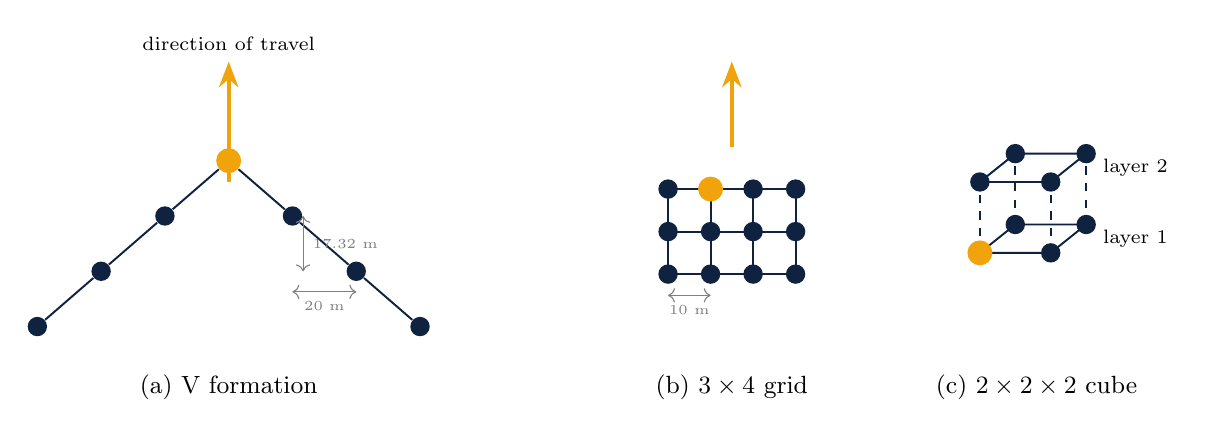
\begin{tikzpicture}[scale=0.9]
  % (a) V formation
  \begin{scope}
    \draw[amber,line width=1.4pt,-{Stealth}] (0,-0.3)--(0,1.4) node[above,font=\scriptsize,black]{direction of travel};
    \node[leader] (L) at (0,0) {};
    \foreach \i in {1,2,3} {
      \node[drone] (l\i) at (-\i*0.9,-\i*0.78) {};
      \node[drone] (r\i) at (\i*0.9,-\i*0.78) {};
    }
    \draw[link] (L)--(l1)--(l2)--(l3); \draw[link] (L)--(r1)--(r2)--(r3);
    \draw[<->,gray,thin] (1.05,-0.78)--(1.05,-1.56) node[midway,right,font=\tiny]{17.32 m};
    \draw[<->,gray,thin] (0.9,-1.85)--(1.8,-1.85) node[midway,below,font=\tiny]{20 m};
    \node[font=\small] at (0,-3.2) {(a) V formation};
  \end{scope}
  % (b) grid
  \begin{scope}[xshift=6.2cm,yshift=-0.4cm]
    \draw[amber,line width=1.4pt,-{Stealth}] (0.9,0.6)--(0.9,1.8);
    \foreach \r in {0,1,2} \foreach \c in {0,1,2,3} {
      \coordinate (g\r\c) at (\c*0.6,-\r*0.6);
    }
    \foreach \r in {0,1,2} { \draw[link] (g\r0)--(g\r3); }
    \foreach \c in {0,1,2,3} { \draw[link] (g0\c)--(g2\c); }
    \foreach \r in {0,1,2} \foreach \c in {0,1,2,3} { \node[drone] at (g\r\c) {}; }
    \node[leader] at (g01) {};
    \draw[<->,gray,thin] (0,-1.5)--(0.6,-1.5) node[midway,below,font=\tiny]{10 m};
    \node[font=\small] at (0.9,-2.8) {(b) $3\times4$ grid};
  \end{scope}
  % (c) cube
  \begin{scope}[xshift=10.6cm,yshift=-1.3cm]
    \foreach \z in {0,1} \foreach \x in {0,1} \foreach \y in {0,1}
      \coordinate (c\x\y\z) at ({\x*1.0+\y*0.5},{\z*1.0+\y*0.4});
    \foreach \z in {0,1} {
      \draw[link] (c00\z)--(c10\z)--(c11\z)--(c01\z)--cycle; }
    \foreach \x in {0,1} \foreach \y in {0,1} { \draw[link,dashed] (c\x\y0)--(c\x\y1); }
    \foreach \z in {0,1} \foreach \x in {0,1} \foreach \y in {0,1} { \node[drone] at (c\x\y\z) {}; }
    \node[leader] at (c000) {};
    \node[font=\scriptsize,right] at (1.6,0.2) {layer 1};
    \node[font=\scriptsize,right] at (1.6,1.2) {layer 2};
    \node[font=\small] at (0.8,-1.9) {(c) $2\times2\times2$ cube};
  \end{scope}
\end{tikzpicture}
\caption{Rigid formations. The amber drone is the leader whose corridor ENHSP plans; lines show
the neighbour links each drone must keep. In the cube, vertical layers are separated by
height.}
\label{fig:vgrid}
\end{figure}

\section{Three-Dimensional Cube Formation}
\paragraph{Mission}
The grid extended into the vertical: a solid block of drones flies one corridor, 10\,m apart
horizontally and vertically (Figure~\ref{fig:vgrid}c). A square footprint is chosen and as many
layers as needed are stacked, allowing a partly filled top layer (for example 9 drones become
$3\times2\times2$ with 9 of 12 cells filled; 25 become $3\times3\times3$). At least eight drones
are needed.

\paragraph{Model}
Layers are separated by height, so each drone has its own \code{target-altitude} (base plus
10\,m per layer), and the run-time route adds a per-drone altitude offset. The swarm climbs
layer by layer, bottom first:

\begin{lstlisting}
(:action open-next-layer
    :parameters (?lo - layer ?hi - layer)
    :precondition (and (layer-below ?lo ?hi) (layer-launched ?lo)
                       (not (layer-launched ?hi))
                       (forall (?d - drone)
                           (or (not (in-layer ?d ?lo)) (at-cruise-altitude ?d))))
    :effect (and (layer-launched ?hi)
                 (forall (?d - drone)
                     (when (in-layer ?d ?hi) (cleared-to-launch ?d)))))
\end{lstlisting}

\noindent Each drone may coordinate with up to 24 neighbours: the $3\times3\times3$ block around
it, except itself and the cells directly above and below. Collision avoidance is structural:
fixed spacing, layer-by-layer ascent and a \code{cube-closed} interlock that must hold before
each leg.

\section{Parabola Formation}
\paragraph{Mission}
Three drones fly side by side on one line across the route, 10\,m apart. The middle drone (the
vertex) cruises at 50\,m and the two arm drones at 60\,m, so seen from behind they form an
upward-opening parabola (Figure~\ref{fig:parabola}). Extra selected drones stay on the ground.

\paragraph{Model}
This plan has the most detailed communication model (Section~\ref{sec:paracomm}). Before any
drone may take its slot, every directed link must be established and each drone must confirm
it is in contact with all of its neighbours. The formation action checks the shape: each arm's
target altitude minus the vertex's must equal \code{arm-rise} (10\,m), so a flat line, an
inverted U or lopsided arms give no plan, and every vertex--arm gap (14.14\,m) must be at least
\code{min-separation} (10\,m).

\begin{lstlisting}
(:action establish-parabola-formation
  :parameters (?vtx - drone ?l - location)
  :precondition (and (formation-leader ?vtx) (slot-vertex ?vtx) (in-formation ?vtx)
     (at ?vtx ?l) (at-cruise-altitude ?vtx) (swarm-comm-ready ?vtx)
     (forall (?a - drone)
       (or (not (arm-drone ?a))
           (and (in-formation ?a) (at ?a ?l) (at-cruise-altitude ?a)
                (= (- (target-altitude ?a) (target-altitude ?vtx)) (arm-rise))
                (>= (link-distance ?vtx ?a) (min-separation))
                (swarm-comm-ready ?a)))))
  :effect (and (parabola-established) (formation-at ?l) (shape-held)))
\end{lstlisting}

\begin{figure}[H]
\centering
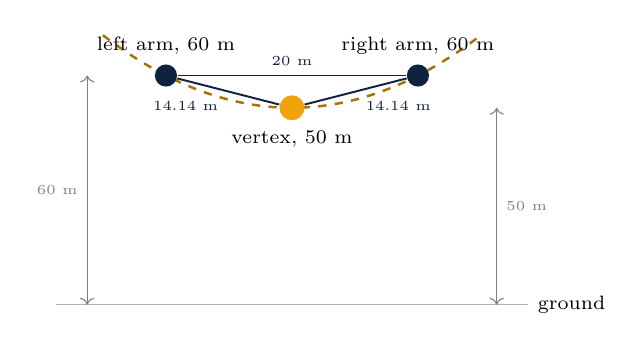
\begin{tikzpicture}[scale=1.0]
  \draw[gray!60] (-3,0)--(3,0) node[right,font=\scriptsize,black]{ground};
  \draw[amber!70!black,dashed,line width=0.9pt,domain=-2.4:2.4,samples=50] plot (\x,{2.5+0.16*\x*\x});
  \node[leader,label={[font=\scriptsize]below:vertex, 50 m}] (v) at (0,2.5) {};
  \node[drone,minimum size=8pt,label={[font=\scriptsize]above:left arm, 60 m}] (a) at (-1.6,2.91) {};
  \node[drone,minimum size=8pt,label={[font=\scriptsize]above:right arm, 60 m}] (b) at (1.6,2.91) {};
  \draw[link] (v)--node[below left,font=\tiny]{14.14 m}(a);
  \draw[link] (v)--node[below right,font=\tiny]{14.14 m}(b);
  \draw[link] (a)--node[above,font=\tiny]{20 m}(b);
  \draw[<->,gray] (2.6,0)--(2.6,2.5) node[midway,right,font=\tiny]{50 m};
  \draw[<->,gray] (-2.6,0)--(-2.6,2.91) node[midway,left,font=\tiny]{60 m};
\end{tikzpicture}
\caption{The parabola formation seen from behind. All three pairs keep a direct link
(full mesh), and every link is within the 100\,m communication range.}
\label{fig:parabola}
\end{figure}

\noindent At run time the vertex corridor is split into legs of at most 200\,m, and the arms are
derived parallel at $\pm10$\,m. All three drones fly one shared timetable, so they arrive at each
waypoint together even though the vertex has 10\,m less to climb.

\section{Figure-Eight Train Formation}
\paragraph{Mission}
The swarm flies a figure-eight in the air as a \emph{train}: one drone behind another along the
curve, 10\,m apart. The operator makes four clicks: a base, then the left end, the crossing point
and the right end of the eight. Each lobe is half a lemniscate of Gerono from the crossing to its
clicked end, so the lobes cross at right angles and may differ in size (Figure~\ref{fig:fig8}).
The drones fly from the base to the crossing along a Dubins path (turn radius at least 25\,m),
fly the requested number of laps, and return to their own landing pads.

\paragraph{Model}
Each drone talks only to the drone directly in front and behind (\code{train-neighbor}). The
leader's lap is planned through nine key waypoints with \code{formation-cruise}, and
\code{follow-leader} moves the followers after every leg. Laps are counted numerically:

\begin{lstlisting}
(:action start-next-lap
  :parameters (?lead - drone ?dest - location ?start - location)
  :precondition (and (lap-end ?dest) (lap-start ?start) (figure8-established)
                     (train-closed) (formation-at ?dest) (train-leader ?lead)
                     (at ?lead ?dest) (< (+ (laps-completed) 1) (laps-required)))
  :effect (and (not (formation-at ?dest)) (formation-at ?start)
               (not (at ?lead ?dest)) (at ?lead ?start)
               (increase (laps-completed) 1)))
\end{lstlisting}

\paragraph{Capacity}
The only place the train can meet itself is the crossing. The train length $(N-1)\times10$\,m
plus 14.1\,m of crossing clearance must therefore fit inside the smaller lobe. This rule is
checked in the GUI before planning, again in the plan worker, and inside PDDL itself as a
precondition of \code{establish-figure8-formation}, so ENHSP refuses an over-full eight.

\begin{figure}[H]
\centering
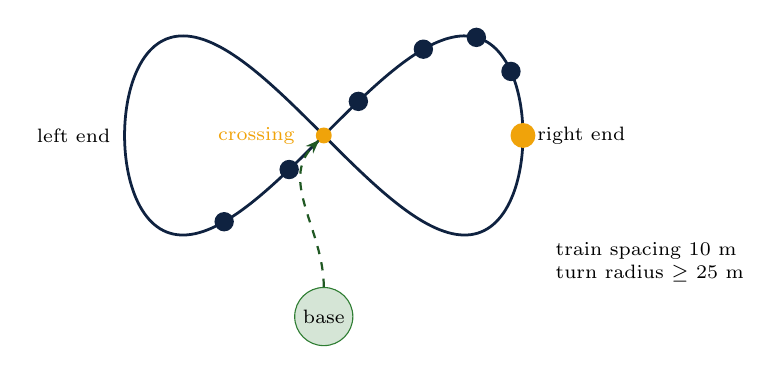
\begin{tikzpicture}[scale=1.15]
  \draw[navy,line width=1.0pt,domain=0:360,samples=120,smooth]
     plot ({2.2*cos(\x)},{1.1*sin(2*\x)});
  \foreach \t in {20,40,60,80,100,120} \node[drone] at ({2.2*cos(\t)},{1.1*sin(2*\t)}) {};
  \node[leader] at ({2.2*cos(0)},{1.1*sin(0)}) {};
  \fill[amber] (0,0) circle (2.5pt) node[left=7pt,font=\scriptsize]{crossing};
  \node[font=\scriptsize,right] at (2.25,0) {right end};
  \node[font=\scriptsize,left] at (-2.25,0) {left end};
  \node[circle,draw=okgreen,fill=okgreen!20,inner sep=2pt,font=\scriptsize] (base) at (0,-2.0) {base};
  \draw[darr,okgreen!70!black] (base) to[out=90,in=-135] (-0.05,-0.05);
  \node[font=\scriptsize,align=left] at (3.6,-1.4) {train spacing 10 m\\turn radius $\geq$ 25 m};
\end{tikzpicture}
\caption{The figure-eight train. The leader (amber) and followers fly the same path one spacing
apart; the base leg joins the eight tangentially at the crossing.}
\label{fig:fig8}
\end{figure}

\section{Star Drone Show}
\paragraph{Mission}
A stationary show around one picked point. The drones take off from pads in rings, spread into a
circle, and then, for each lap, form a star, return to the circle, spin the circle once, form the
star again, spin the star and return to the circle, before landing on their own pads
(Figure~\ref{fig:shows}a). Six or seven drones make a 3-pointed star, eight or nine a 4-pointed
star, and ten or more a 5-pointed star; 6 to 40 drones are allowed.

\paragraph{Model}
ENHSP sequences \code{form-circle}, then per lap \code{form-star}, \code{form-circle-in-lap},
\code{spin-circle}, \code{form-star-again}, \code{spin-star} and \code{close-lap}, and finally
\code{land-show}. The plan worker checks that exactly this sequence is returned. Every drone keeps
the same order round the centre in the circle and the star, so shape changes never cross paths;
the show is sized until all drones are at least 10\,m apart in each shape and at least 9\,m apart
during transitions.

\section{Planetary Orbit Show}
\paragraph{Mission}
A solar-system show round one picked point (the sun), with 2 to 8 drones, one per planet. Drone
$k$ orbits at a radius of $50(k+1)$\,m, and neighbouring orbits turn in opposite directions
(Figure~\ref{fig:shows}b). One lap is one turn of the outermost drone; inner drones make as many
whole turns as fit, so all drones line up again on the north line at the end of every lap.

\paragraph{Model}
\code{enter-orbits} may fire only when every drone has climbed and has \code{neighbor-comm-ok},
and only if every pair of orbit neighbours turns in opposite directions:

\begin{lstlisting}
(forall (?a - drone ?b - drone)
    (or (not (orbit-neighbor ?a ?b))
        (and (orbits-clockwise ?a) (orbits-anticlockwise ?b))
        (and (orbits-anticlockwise ?a) (orbits-clockwise ?b))))
\end{lstlisting}

\noindent One \code{fly-lap} follows per lap, counted by \code{laps-completed}, then
\code{land-planets}.

\begin{figure}[H]
\centering
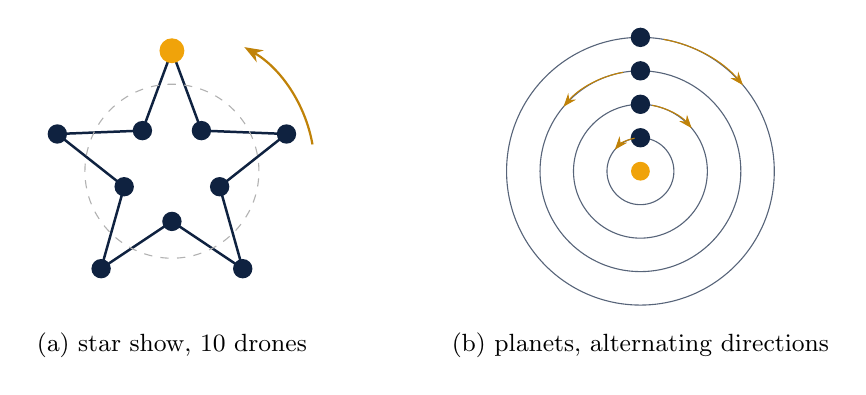
\begin{tikzpicture}[scale=0.85]
  \begin{scope}
    \foreach \k in {0,...,9} {
      \pgfmathsetmacro{\r}{ifthenelse(mod(\k,2)==0,1.8,0.75)}
      \coordinate (s\k) at ({90+\k*36}:\r);
    }
    \draw[navy,line width=0.9pt] (s0)--(s1)--(s2)--(s3)--(s4)--(s5)--(s6)--(s7)--(s8)--(s9)--cycle;
    \draw[gray!60,dashed] (0,0) circle (1.3);
    \foreach \k in {0,...,9} \node[drone] at (s\k) {};
    \node[leader] at (s0) {};
    \draw[amber!80!black,-{Stealth},line width=0.8pt] (2.1,0.4) arc (10:60:2.1);
    \node[font=\small] at (0,-2.6) {(a) star show, 10 drones};
  \end{scope}
  \begin{scope}[xshift=7cm]
    \fill[amber] (0,0) circle (4pt);
    \foreach \k/\dir in {1/1,2/-1,3/1,4/-1} {
      \draw[navy!70] (0,0) circle (\k*0.5);
      \node[drone] at (90:\k*0.5) {};
      \ifnum\dir=1
        \draw[-{Stealth},amber!80!black] (100:\k*0.5) arc (100:140:\k*0.5);
      \else
        \draw[-{Stealth},amber!80!black] (80:\k*0.5) arc (80:40:\k*0.5);
      \fi
    }
    \node[font=\small] at (0,-2.6) {(b) planets, alternating directions};
  \end{scope}
\end{tikzpicture}
\caption{Shape-changing shows. Both are flown against a shared timetable so that every phase
starts and ends together for all drones.}
\label{fig:shows}
\end{figure}

\section{Road Inspection}
\paragraph{Mission}
The operator clicks a source and a destination on a road. One drone takes off at the source,
follows the road's exact path to the destination, flies the same road back and lands at the
source. The road geometry comes from an OSRM routing server on OpenStreetMap
data~\cite{luxen2011osrm}.

\paragraph{Model}
The road is split into at most 12 segments, each with its own length and energy. ENHSP plans
\code{inspect-segment} for each in order, \code{finish-inspection} at the destination,
\code{return-along-road} back segment by segment, and \code{land-at-source}. Each segment
inspection checks GPS, communication, health and that the battery covers the segment. If no road
route exists, a click is more than 30\,m from any road, or the two points are less than 20\,m
apart along the road, the plan fails before anything flies.

\section{Summary of the Plans}
Table~\ref{tab:plansummary} compares the ten plans.

\begin{table}[!htb]
\caption{Comparison of the mission plans}\label{tab:plansummary}
\small
\begin{tabularx}{\textwidth}{@{}lP{0.2\textwidth}P{0.22\textwidth}Y@{}}
\toprule
\textbf{Plan} & \textbf{Map input} & \textbf{What ENHSP plans} & \textbf{Special feature} \\
\midrule
Travel     & source, destination, no-fly area & every drone's legs & full controller fault responses \\
Search     & base, forest polygon & one lane per drone & pairwise separation check \\
V          & source, destination, no-fly area & leader corridor & timed wing launch \\
Grid       & as V & leader corridor & 4-neighbour links \\
Cube       & as V & leader corridor & layer-by-layer ascent \\
Parabola   & as V & vertex corridor & range-checked link mesh, shape check \\
Figure-8   & base and three points & leader's lap & capacity rule, laps \\
Star       & one point & show phases & circle/star/spin sequence \\
Planets    & one point & show phases & opposite-direction orbits \\
Inspect    & two points on a road & road segments & OSRM road geometry \\
\bottomrule
\end{tabularx}
\end{table}

%% =====================================================================
%%  CHAPTER 6  COMMUNICATION
%% =====================================================================
\chapter{Inter-Drone Communication}\label{ch:comm}
Communication appears at two levels in the simulator. In the PDDL models it is a set of
conditions: a drone may only act if its links are up. At run time it is a real exchange of
messages between the ground station and the drones. This chapter explains both and how they
relate.

\section{Communication in the PDDL Models}
Two flags carry communication state for every drone:
\begin{itemize}
  \item \code{communication-ok}: the link between the drone and the ground controller works;
  \item \code{neighbor-comm-ok}: the drone's links to its formation neighbours work.
\end{itemize}
Every action that moves a drone or changes the formation checks the relevant flags. A formation
cannot be established, cruise a leg or close up if any member has lost its neighbour links.
Each plan also declares \emph{who} must talk to whom, using a neighbour relation suited to its
shape (Table~\ref{tab:neighbors}, Figure~\ref{fig:topologies}).

\begin{table}[H]
\caption{Neighbour relations declared by each formation}\label{tab:neighbors}
\small
\begin{tabularx}{\textwidth}{@{}l>{\ttfamily\footnotesize}lY@{}}
\toprule
\textbf{Plan} & \textbf{\normalfont\small Relation} & \textbf{Who talks to whom} \\
\midrule
V formation & wing-neighbor   & leader with rank 1, then rank to rank along each wing (a chain) \\
Grid        & grid-neighbor   & up to 4 neighbours: front, back, left, right \\
Cube        & cube-neighbor   & up to 24 neighbours in the surrounding $3\times3\times3$ block,
excluding directly above and below \\
Parabola    & parabola-neighbor & all three pairs, in both directions (6 directed links) \\
Figure-8    & train-neighbor  & the drone in front and the drone behind \\
Planets     & orbit-neighbor  & drones on adjacent orbits \\
\bottomrule
\end{tabularx}
\end{table}

\begin{figure}[H]
\centering
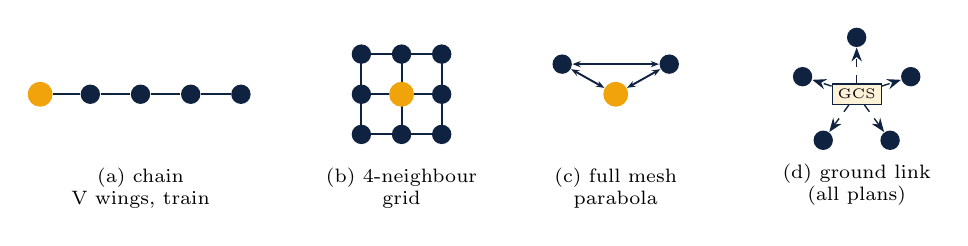
\begin{tikzpicture}[scale=0.85]
  % chain
  \begin{scope}
    \node[leader] (c0) at (0,0) {};
    \foreach \i in {1,...,4} \node[drone] (c\i) at (\i*0.75,0) {};
    \draw[link] (c0)--(c1)--(c2)--(c3)--(c4);
    \node[font=\scriptsize,align=center] at (1.5,-1.4) {(a) chain\\V wings, train};
  \end{scope}
  % grid 4-neighbour
  \begin{scope}[xshift=4.8cm,yshift=0.6cm]
    \foreach \r in {0,1,2} \foreach \c in {0,1,2} \coordinate (q\r\c) at (\c*0.6,-\r*0.6);
    \foreach \r in {0,1,2} \draw[link] (q\r0)--(q\r2);
    \foreach \c in {0,1,2} \draw[link] (q0\c)--(q2\c);
    \foreach \r in {0,1,2} \foreach \c in {0,1,2} \node[drone] at (q\r\c) {};
    \node[leader] at (q11) {};
    \node[font=\scriptsize,align=center] at (0.6,-2.0) {(b) 4-neighbour\\grid};
  \end{scope}
  % full mesh
  \begin{scope}[xshift=8.6cm]
    \node[leader] (m0) at (0,0) {};
    \node[drone] (m1) at (-0.8,0.45) {};
    \node[drone] (m2) at (0.8,0.45) {};
    \draw[link,{Stealth[length=3pt]}-{Stealth[length=3pt]}] (m0)--(m1);
    \draw[link,{Stealth[length=3pt]}-{Stealth[length=3pt]}] (m0)--(m2);
    \draw[link,{Stealth[length=3pt]}-{Stealth[length=3pt]}] (m1)--(m2);
    \node[font=\scriptsize,align=center] at (0,-1.4) {(c) full mesh\\parabola};
  \end{scope}
  % ground star
  \begin{scope}[xshift=12.2cm]
    \node[rectangle,draw=navy,fill=softamber,font=\tiny,inner sep=2pt] (g) at (0,0) {GCS};
    \foreach \a in {0,72,144,216,288} { \node[drone] (s\a) at (\a+90:0.85) {}; \draw[darr,line width=0.5pt] (g)--(s\a); }
    \node[font=\scriptsize,align=center] at (0,-1.35) {(d) ground link\\(all plans)};
  \end{scope}
\end{tikzpicture}
\caption{Communication topologies. (a)--(c) are drone-to-drone relations declared in PDDL;
(d) is the ground-controller link represented by \code{communication-ok}.}
\label{fig:topologies}
\end{figure}

\section{The Range-Checked Link Model of the Parabola Plan}\label{sec:paracomm}
In most plans the links are summarised by the per-drone flag. The parabola plan models each
directed link explicitly. A link from $d_1$ to $d_2$ can be established only when both drones
are airborne at cruise altitude, both radios work, and the straight-line distance between them
is within the communication range of 100\,m:

\begin{lstlisting}
(:action establish-comm-link
    :parameters (?d1 - drone ?d2 - drone)
    :precondition (and (parabola-neighbor ?d1 ?d2) (not (link-up ?d1 ?d2))
                       (airborne ?d1) (airborne ?d2)
                       (at-cruise-altitude ?d1) (at-cruise-altitude ?d2)
                       (communication-ok ?d1) (communication-ok ?d2)
                       (neighbor-comm-ok ?d1) (neighbor-comm-ok ?d2)
                       (<= (link-distance ?d1 ?d2) (comm-range)))
    :effect (link-up ?d1 ?d2))
\end{lstlisting}

\noindent A drone becomes \code{swarm-comm-ready} through \code{confirm-swarm-comm} once it has
a link to every one of its neighbours (a universally quantified condition). Only then can it
take its slot. During flight, \code{hold-parabola-shape} requires every declared link to still be
up, and if a drone loses its neighbour links, \code{detect-neighbor-link-loss} removes all links
to and from that drone, so the shape cannot be re-formed until they are restored. A negative test
with the range reduced to 15\,m (below the 20\,m arm-to-arm distance) correctly produced no plan.
In the solved plan, the six \code{establish-comm-link} actions and three
\code{confirm-swarm-comm} actions appear right after the climbs and before any slot is taken
(Section~\ref{sec:sampleplan}).

\section{Run-Time Communication between Ground Station and Drones}
At run time each drone is an independent thread that owns its state. It can only be reached
through a command inbox and only reports through a telemetry callback. Over the network, the
ground station and drones use a simple JSON-over-UDP protocol, one datagram per message, designed
so that it can later be replaced by MAVLink~\cite{mavlink}. Every message carries the drone's
MAVLink SYSID, so one ground socket can address the whole swarm
(Figure~\ref{fig:udp}).

\begin{figure}[H]
\centering
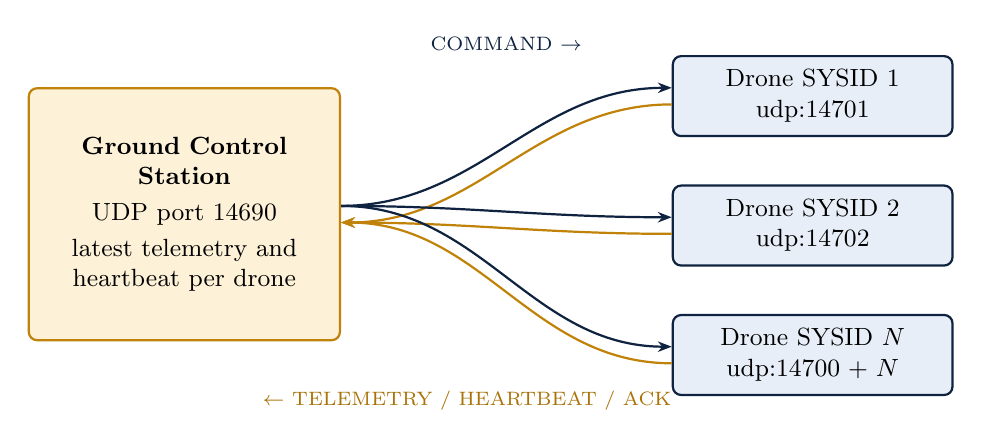
\begin{tikzpicture}[node distance=6mm]
  \node[abox,text width=3.6cm,minimum height=3.2cm] (gcs) {\textbf{Ground Control}\\\textbf{Station}\\[2pt]UDP port 14690\\[2pt]
     latest telemetry and heartbeat per drone};
  \node[box,right=4.2cm of gcs,yshift=1.5cm,text width=3.2cm] (d1) {Drone SYSID 1\\udp:14701};
  \node[box,below=6mm of d1,text width=3.2cm] (d2) {Drone SYSID 2\\udp:14702};
  \node[box,below=6mm of d2,text width=3.2cm] (dn) {Drone SYSID $N$\\udp:$14700+N$};
  \foreach \d in {d1,d2,dn} {
    \draw[arr] ([yshift=3pt]gcs.east) to[out=0,in=180] node[pos=0.55,above,font=\tiny,sloped]{} ([yshift=3pt]\d.west);
    \draw[arr,amber!80!black] ([yshift=-3pt]\d.west) to[out=180,in=0] ([yshift=-3pt]gcs.east);
  }
  \node[font=\scriptsize,navy,align=center] at ($(gcs.north east)!0.5!(d1.north west)+(0,0.35)$) {COMMAND $\rightarrow$};
  \node[font=\scriptsize,amber!70!black,align=center] at ($(gcs.south east)+(1.6,-0.75)$) {$\leftarrow$ TELEMETRY / HEARTBEAT / ACK};
\end{tikzpicture}
\caption{Run-time messaging. Commands are routed to a port derived from each drone's SYSID;
every drone reports back to one ground station socket.}
\label{fig:udp}
\end{figure}

\noindent Table~\ref{tab:commands} lists the commands. A drone sends a heartbeat every second
and telemetry every 0.5\,s. The ground station treats a drone as out of contact if no heartbeat
arrives for 3\,s. On the drone side, if nothing is heard from the ground for more than 5\,s the
drone marks its link \code{DEGRADED}, and after 10\,s \code{LOST}. Link loss is therefore
\emph{observed} from missing messages rather than assumed.

\begin{table}[H]
\caption{Commands of the ground-station-to-drone protocol}\label{tab:commands}
\small
\begin{tabularx}{\textwidth}{@{}>{\ttfamily\footnotesize}P{0.28\textwidth}Y@{}}
\toprule
\textbf{\normalfont\small Command} & \textbf{Purpose} \\
\midrule
NAVIGATE & The one mission operation: upload a whole route (approach, loop, laps, depart). \\
ARM, DISARM, TAKEOFF, LAND & Basic flight control. \\
HOLD, RESUME & Pause and continue the mission (used while the operator decides on a fault). \\
RETURN\_TO\_LAUNCH, ABORT & Fall back to the start point, or stop. \\
SET\_GPS & Fault injection: switch the drone's GPS fix off or on. \\
SET\_SPEED & Change cruise speed in flight. \\
TRAIN\_PACE & Formation keeping: the shared, time-stamped pace of the train or show clock. \\
PING, SHUTDOWN & Liveness check and stop the drone thread. \\
\bottomrule
\end{tabularx}
\end{table}

\section{On-Board Formation Keeping}
Early versions of the figure-eight plan let the ground station correct each drone against its
neighbours' live positions. Because speed commands arrived two or three polls late, which is many
metres of flight at the simulator's time scale, a train of drones each over-correcting to the one
in front began to oscillate, and drones bunched and overtook each other. The fix moved formation
keeping on board (Figure~\ref{fig:pace}). The ground station now only broadcasts a shared,
time-stamped \code{TRAIN\_PACE}. Every tick, each drone works out where it should be (the pace
extrapolated from its time stamp, minus its place in the train), measures its own exact progress
along its own route, and sets its own autopilot speed to close the gap. Neighbour information is
still used, but only as a cap: if the drone in front is reported too close, the drone does not
speed up into it; if a drone falls behind, the ground station slows the pace so the train waits.

For the star and planets shows the same mechanism runs in \emph{schedule} mode: each drone gets
keyframes ``at clock time $t$, be $s$ metres along your route'', and the pace is a shared clock.
Every drone flying its own timetable against one clock is what makes every shape change start and
finish together.

\begin{figure}[H]
\centering
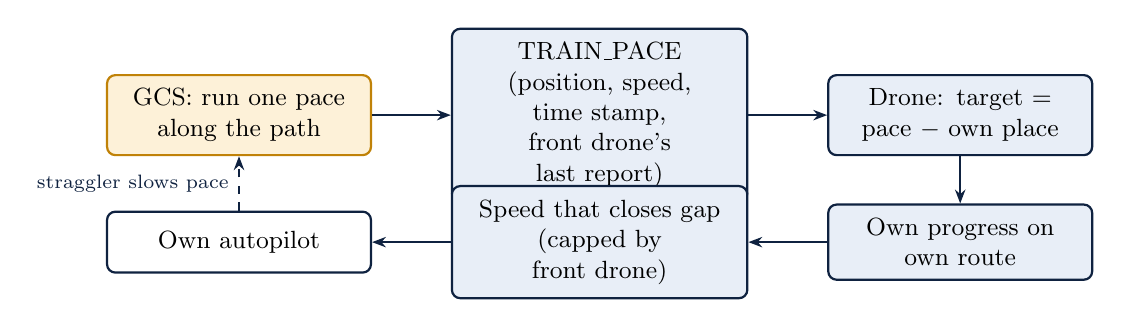
\begin{tikzpicture}[node distance=6mm and 10mm]
  \node[abox,text width=3.0cm] (gcs) {GCS: run one pace\\along the path};
  \node[box,right=of gcs,text width=3.4cm] (msg) {TRAIN\_PACE\\(position, speed, time stamp,\\front drone's last report)};
  \node[box,right=of msg,text width=3.0cm] (drone) {Drone: target =\\pace $-$ own place};
  \node[box,below=of drone,text width=3.0cm] (me) {Own progress on\\own route};
  \node[box,left=of me,text width=3.4cm] (spd) {Speed that closes gap\\(capped by front drone)};
  \node[gbox,left=of spd,text width=3.0cm] (ap) {Own autopilot};
  \draw[arr] (gcs)--(msg); \draw[arr] (msg)--(drone); \draw[arr] (drone)--(me);
  \draw[arr] (me)--(spd); \draw[arr] (spd)--(ap);
  \draw[darr] (ap.north)--node[left,font=\scriptsize]{straggler slows pace}(gcs.south);
\end{tikzpicture}
\caption{On-board formation keeping. Only the pace is sent from the ground; each drone closes its
own gap every tick.}
\label{fig:pace}
\end{figure}

\section{How the Two Levels Relate}
The PDDL flags are a \emph{planning-time} statement: the plan is only valid under the assumption
that the listed links work. The run-time protocol is what actually carries commands and reports.
The two are connected through the fault events of Chapter~\ref{ch:faults}: when the run time
observes a fault, the mission is held and the operator decides how to continue. The PDDL
conditions do not by themselves monitor real radio links; this distinction is discussed in
Chapter~\ref{ch:discussion}.

%% =====================================================================
%%  CHAPTER 7  FAULTS AND BATTERY HEALTH
%% =====================================================================
\chapter{Fault Modelling and Battery Health}\label{ch:faults}

\section{Faults Modelled in PDDL}
Every domain includes the same family of detection actions. Each one fires for a flying drone
whose health flag has failed, records a failure state, and takes the drone out of flight and,
in formation plans, out of the formation. Table~\ref{tab:faults} lists them.

\begin{table}[H]
\caption{Fault detection actions shared by the domains}\label{tab:faults}
\small
\begin{tabularx}{\textwidth}{@{}>{\ttfamily\footnotesize}P{0.27\textwidth}P{0.25\textwidth}Y@{}}
\toprule
\textbf{\normalfont\small Action} & \textbf{Fires when} & \textbf{Effect} \\
\midrule
detect-gps-loss & flying and not \code{gps-ok} & \code{gps-lost}; not flying; leaves the
formation (travel also sets \code{gps-warning}) \\
detect-communication-loss & flying and not \code{communication-ok} & \code{communication-lost};
not flying; leaves the formation; parabola also clears \code{swarm-comm-ready} \\
detect-neighbor-link-loss & flying and not \code{neighbor-comm-ok} (formation plans) &
\code{communication-lost}; leaves the formation; parabola also drops every link to and from the
drone \\
detect-health-failure & flying and \code{health} $<$ \code{minimum-health} (40) &
\code{health-failure}; not flying; leaves the formation \\
notify-ground-controller & any of the three failure states & \code{controller-notified} \\
\bottomrule
\end{tabularx}
\end{table}

The GPS loss detection, for example, is:

\begin{lstlisting}
(:action detect-gps-loss
    :parameters (?d - drone)
    :precondition (and (flying ?d) (not (gps-ok ?d)))
    :effect (and (gps-lost ?d) (not (flying ?d)) (not (in-formation ?d))))
\end{lstlisting}

\noindent Because every movement and formation action also requires \code{gps-ok},
\code{communication-ok}, \code{drone-healthy} and, for formations, \code{neighbor-comm-ok}, a
problem that starts with a failed flag has no plan that moves the affected drone. The planner
thus refuses to fly an unhealthy drone, and a failed member blocks the formation actions that
depend on it.

\section{Ground Controller Responses}
The point-to-point domain goes further and models what the ground controller can order once it
has been notified (Figure~\ref{fig:faultflow}):
\begin{itemize}
  \item \textbf{Return}: \code{controller-order-return} sets \code{emergency-return}, and
        \code{return-to-source} flies the drone back over a safe route, provided the battery
        covers the return leg.
  \item \textbf{Hover}: \code{controller-order-hover} puts the drone in a hover. The \code{hover}
        action drains \code{hover-energy} while the battery stays above the return reserve; when
        it reaches the reserve, \code{initiate-low-battery-return} switches the drone to an
        emergency return.
  \item \textbf{Sacrifice}: \code{sacrifice-drone} lands the drone immediately where it is when the
        controller decides it cannot be recovered.
\end{itemize}

\begin{figure}[H]
\centering
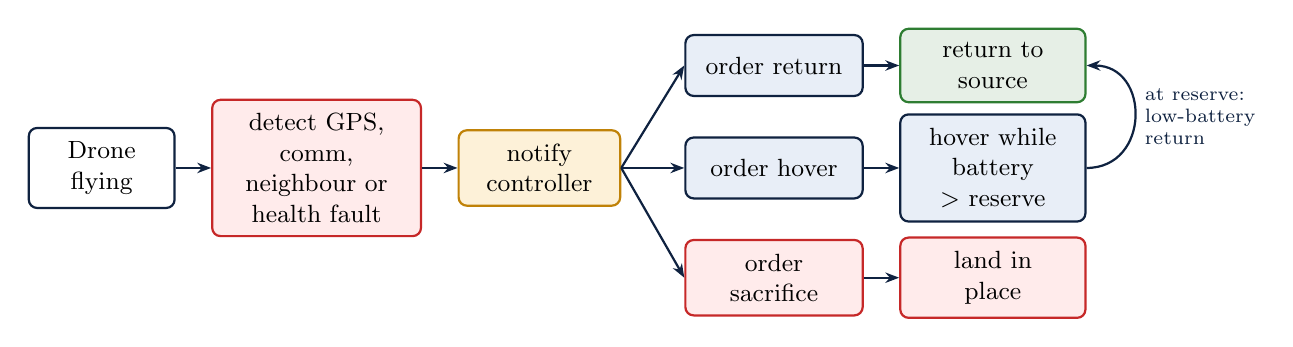
\begin{tikzpicture}[node distance=5mm and 4.5mm, every node/.style={font=\footnotesize}]
  \node[box,fill=white,text width=1.5cm] (fl) {Drone\\flying};
  \node[box,fill=red!8,draw=warnred,right=of fl,text width=2.3cm] (det) {detect GPS, comm,\\neighbour or\\health fault};
  \node[abox,right=of det,text width=1.7cm] (not) {notify\\controller};
  \node[box,right=8mm of not,text width=1.9cm] (hov) {order hover};
  \node[box,above=of hov,text width=1.9cm] (ret) {order return};
  \node[box,below=of hov,text width=1.9cm,fill=red!8,draw=warnred] (sac) {order sacrifice};
  \node[box,right=of hov,text width=2.0cm] (low) {hover while\\battery $>$ reserve};
  \node[box,fill=okgreen!12,draw=okgreen,right=of ret,text width=2.0cm] (src) {return to\\source};
  \node[box,right=of sac,text width=2.0cm,fill=red!8,draw=warnred] (land) {land in\\place};
  \draw[arr] (fl)--(det); \draw[arr] (det)--(not);
  \draw[arr] (not.east)--(ret.west); \draw[arr] (not)--(hov); \draw[arr] (not.east)--(sac.west);
  \draw[arr] (ret)--(src); \draw[arr] (hov)--(low); \draw[arr] (sac)--(land);
  \draw[arr] (low.east) to[out=0,in=0,looseness=1.6] node[right,font=\scriptsize,align=left]{at reserve:\\low-battery\\return} (src.east);
\end{tikzpicture}
\caption{Fault handling in the point-to-point domain: detection, notification and the three
controller responses.}
\label{fig:faultflow}
\end{figure}

\section{Battery as a Planning Resource}
Battery is a numeric fluent in every domain, in model units with 100 as a full charge. It is used
in three ways.

\paragraph{Energy per leg}
Each leg has an \code{energy-required} value. When a template is retargeted, this value is
recomputed from the new leg length at the leg's own energy-per-metre rate, with a default of
0.0125 units per metre (12.5 units per kilometre). Every move requires the battery to be
strictly greater than the leg's cost and decreases it by that cost.

\paragraph{Climb, cruise and hover energy}
Formation plans charge \code{climb-energy} for the climb to cruise altitude (in the parabola
plan 4 units for the vertex and 5 for the arms, which climb 10\,m further), and
\code{cruise-leg-energy} (12 units) for each follower or arm leg. The travel domain charges
\code{hover-energy} for each hover step.

\paragraph{Reserve for return}
Every drone keeps a \code{minimum-return-battery} of 30 units. \code{pre-flight-check} refuses a
drone whose battery is not above this reserve, \code{check-battery} and
\code{notify-insufficient-battery} classify each leg as affordable or not, and the hover and
search domains switch to a return when the battery reaches the reserve. Health is a separate
numeric score (100 initially, minimum 40), so a drone can be refused for poor health even with a
full battery.

\section{Battery Health at Run Time}
During flight each drone thread integrates its own battery. With the default settings a drone has
a 5\,200\,mAh battery and draws a nominal 20\,A in flight; its percentage is computed from the
consumed charge. The drone classifies its own health from the battery and the GPS fix
(Figure~\ref{fig:battery}): \code{NOMINAL} above 20\,\%, \code{DEGRADED} at or below 20\,\% or
without GPS, \code{CRITICAL} at or below 5\,\%, and \code{FAILED} if the battery is exhausted in
flight, in which case the drone is lost.

\begin{figure}[H]
\centering
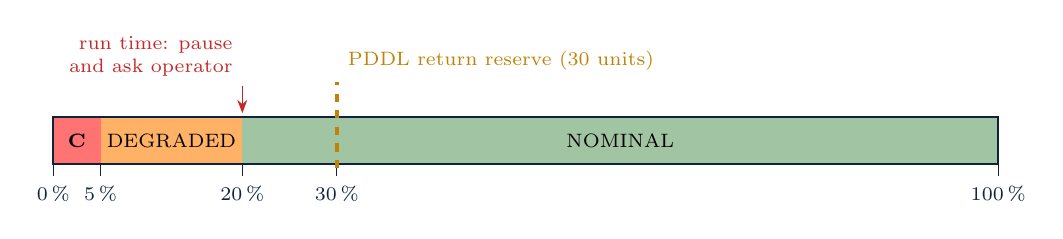
\begin{tikzpicture}
  \def\W{12}
  \fill[red!55]      (0,0) rectangle (0.05*\W,0.6);
  \fill[orange!60]   (0.05*\W,0) rectangle (0.20*\W,0.6);
  \fill[okgreen!45]  (0.20*\W,0) rectangle (\W,0.6);
  \draw[navy,line width=0.8pt] (0,0) rectangle (\W,0.6);
  \foreach \p/\l in {0/0\,\%,0.05/5\,\%,0.20/20\,\%,0.30/30\,\%,1/100\,\%}
    \draw[navy] (\p*\W,0)--(\p*\W,-0.15) node[below,font=\scriptsize]{\l};
  \node[font=\scriptsize] at (0.025*\W,0.3) {\textbf{C}};
  \node[font=\scriptsize] at (0.125*\W,0.3) {DEGRADED};
  \node[font=\scriptsize] at (0.6*\W,0.3) {NOMINAL};
  \draw[amber!80!black,line width=1.4pt,dashed] (0.30*\W,-0.05)--(0.30*\W,1.05)
     node[above right,font=\scriptsize,align=left]{PDDL return reserve (30 units)};
  \draw[-{Stealth},warnred] (0.20*\W,1.0) node[above left,font=\scriptsize,align=right,text=warnred]{run time: pause\\and ask operator}--(0.20*\W,0.65);
\end{tikzpicture}
\caption{Battery thresholds. Below the bar: run-time health classes (C = CRITICAL; FAILED at
0\,\% in flight). The planner keeps a 30-unit reserve; at 20\,\% the run time holds the swarm
and asks the operator.}
\label{fig:battery}
\end{figure}

\noindent When any drone crosses the low-battery threshold, the ground station \emph{pauses the
whole mission} so that the drones do not drain while the operator decides; at the compressed time
scale the decision window would otherwise be a fraction of a second. A dialog shows the drone's
battery and the nearest landing point, with a note whether it is within reach on the remaining
charge. The operator may divert and land now, or press on, in which case the drone will be lost
when the battery runs flat. A drone whose battery reaches zero in flight is reported as lost and
sacrificed.

\section{Fault Injection and Operator Decisions}
The GUI's fault injection panel lets the operator target one or more drones by SYSID with a
fault type (GPS loss, communications loss or battery failure), a severity and a duration
(zero meaning until reset). In the thread-based backend, GPS loss is delivered as a
\code{SET\_GPS} command, so the drone itself loses its fix. On GPS loss the ground station holds
the swarm and asks the operator whether the drone should fall back to its start point and land,
showing the distance back and whether the remaining charge covers it; otherwise the drone holds
position until GPS returns, while its battery keeps draining. When GPS is reacquired the mission
resumes. Table~\ref{tab:faultmap} maps each fault to its PDDL model and run-time behaviour.

\begin{table}[H]
\caption{Faults: how each is modelled in PDDL and handled at run time}\label{tab:faultmap}
\small
\begin{tabularx}{\textwidth}{@{}P{0.17\textwidth}P{0.32\textwidth}Y@{}}
\toprule
\textbf{Fault} & \textbf{PDDL model} & \textbf{Run-time behaviour} \\
\midrule
GPS loss & not \code{gps-ok}; \code{detect-gps-loss} & injected with \code{SET\_GPS}; drone
\code{DEGRADED}; swarm held; operator chooses fall-back or hold \\
Communication loss & not \code{communication-ok}; \code{detect-communication-loss} & observed
from missing heartbeats and contact (\code{DEGRADED} after 5\,s, \code{LOST} after 10\,s) \\
Neighbour link loss & not \code{neighbor-comm-ok}; \code{detect-neighbor-link-loss} & reflected
in formation keeping through the front-drone cap and pace slowing \\
Health failure & \code{health} below \code{minimum-health}; \code{detect-health-failure} &
drone health classes \code{NOMINAL}/\code{DEGRADED}/\code{CRITICAL}/\code{FAILED} \\
Low battery & battery not above reserve; \code{notify-insufficient-battery},
\code{initiate-low-battery-return} & at 20\,\% swarm paused, operator chooses emergency landing
or press on; at 0\,\% drone lost \\
\bottomrule
\end{tabularx}
\end{table}

%% =====================================================================
%%  CHAPTER 8  RESULTS
%% =====================================================================
\chapter{Verification and Results}\label{ch:results}

\section{Method}
Each plan was verified in two ways. First, ENHSP was run directly on problems produced by the real
expand, retarget and solve pipeline, for a range of drone counts. Second, the resulting routes were
flown headless through the real drone threads and simulated firmware, and the spacing, altitudes
and landing positions were measured. Negative tests were added where a plan must refuse a
problem. The run logs in \code{plans/*/runs/} record the in-app requests.

\section{In-App Planning Requests}
Table~\ref{tab:runs} summarises the logged requests for the four longest-running plans. Every
unsolvable travel and V request was traced to an infeasible combination of source, destination
and no-fly area, where no safe path existed. The grid failures all occurred in a short window
before a template fix (Section~\ref{sec:defects}); every grid request after the fix solved.

\begin{table}[H]
\caption{Logged planning requests per plan}\label{tab:runs}
\small
\begin{tabularx}{\textwidth}{@{}lrrrY@{}}
\toprule
\textbf{Plan} & \textbf{Runs} & \textbf{Solved} & \textbf{Unsolvable} & \textbf{Notes} \\
\midrule
Forest search & 69 & 69 & 0 & no failures on record \\
Travel        & 83 & 76 & 7 & infeasible no-fly inputs during early testing \\
V formation   & 65 & 62 & 2 & 2 infeasible inputs; 1 run closed mid-plan \\
Grid          & 19 & 15 & 4 & all 4 before the hover-altitude fix \\
\bottomrule
\end{tabularx}
\end{table}

\section{Scalability of the Cube Formation}
Table~\ref{tab:cube} and Figure~\ref{fig:cubeplot} show planning time and plan length for the
cube formation. Plan length grows linearly with the number of drones, about four actions per
drone. Planning time stays below 4\,s up to 36 drones and reaches 50\,s for a full $4\times4\times4$
block of 64 drones. A launch-order audit of the 25-drone plan found no drone taking off before
its layer opened and no layer opening before the one below had finished climbing.

\begin{table}[H]
\caption{Cube formation: ENHSP results through the real pipeline}\label{tab:cube}
\small
\begin{tabular*}{\textwidth}{@{\extracolsep{\fill}}lrrrrrrrr@{}}
\toprule
\textbf{Drones} & 8 & 9 & 12 & 16 & 25 & 27 & 36 & 64 \\
\textbf{Shape} & $2{\times}2{\times}2$ & $3{\times}2{\times}2$ & $2{\times}3{\times}3$ & $2{\times}3{\times}3$ &
 $3{\times}3{\times}3$ & $3{\times}3{\times}3$ & $3{\times}4{\times}4$ & $4{\times}4{\times}4$ \\
\midrule
Time (s) & 0.4 & 0.5 & 0.6 & 0.7 & 1.2 & 1.8 & 3.4 & 50.0 \\
Plan length & 42 & 47 & 58 & 74 & 111 & 119 & 155 & 268 \\
\bottomrule
\end{tabular*}
\end{table}

\begin{figure}[H]
\centering
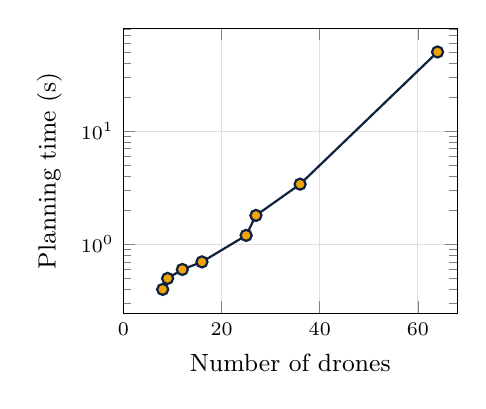
\begin{tikzpicture}
\begin{axis}[
  width=0.48\textwidth,height=5.2cm,
  xlabel={Number of drones},ylabel={Planning time (s)},
  ymode=log,log basis y=10,
  grid=major,grid style={gray!25},
  tick label style={font=\scriptsize},label style={font=\small},
  xmin=0,xmax=68,
]
\addplot[navy,thick,mark=*,mark options={fill=amber,draw=navy}] coordinates
  {(8,0.4)(9,0.5)(12,0.6)(16,0.7)(25,1.2)(27,1.8)(36,3.4)(64,50.0)};
\end{axis}
\end{tikzpicture}\hfill
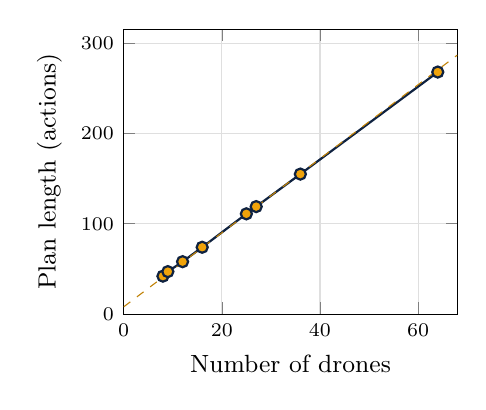
\begin{tikzpicture}
\begin{axis}[
  width=0.48\textwidth,height=5.2cm,
  xlabel={Number of drones},ylabel={Plan length (actions)},
  grid=major,grid style={gray!25},
  tick label style={font=\scriptsize},label style={font=\small},
  xmin=0,xmax=68,ymin=0,
]
\addplot[navy,thick,mark=*,mark options={fill=amber,draw=navy}] coordinates
  {(8,42)(9,47)(12,58)(16,74)(25,111)(27,119)(36,155)(64,268)};
\addplot[amber!80!black,dashed,domain=0:68] {4.1*x+8};
\end{axis}
\end{tikzpicture}
\caption{Cube formation scalability. Left: planning time (log scale). Right: plan length, close to
linear in the number of drones (dashed line $\approx 4.1N + 8$).}
\label{fig:cubeplot}
\end{figure}

\section{Figure-Eight Capacity and Flight Quality}
On an asymmetric eight with lobes of 337\,m and 281\,m, the computed capacity was 27 drones. ENHSP
solved every count up to 27 and returned no plan for 28, in agreement with the Python check
(Table~\ref{tab:fig8}). With a full 27-drone train, the minimum distance between any two drones at
any waypoint step was 9.85\,m, including at the crossing. Ten drones with 20 laps solved in 0.8\,s,
because laps are counted in PDDL and flown on board with a single repeat instruction rather than
being unrolled.

\begin{table}[H]
\caption{Figure-eight train: ENHSP results on an eight of capacity 27}\label{tab:fig8}
\small
\begin{tabular*}{\textwidth}{@{\extracolsep{\fill}}lrrrrrr@{}}
\toprule
\textbf{Drones} & 2 & 5 & 12 & 25 & 27 & 28 \\
\midrule
Time (s) & 0.4 & 0.4 & 0.7 & 2.7 & 3.3 & -- \\
Plan length & 26 & 38 & 66 & 118 & 126 & no plan (as intended) \\
\bottomrule
\end{tabular*}
\end{table}

\noindent After formation keeping moved on board (Chapter~\ref{ch:comm}), a replay of a logged
16-drone, 2-lap run changed from a median neighbour gap of 23.7\,m with a minimum of 0.0\,m
(collisions) to a median of 10.0\,m, with 90\,\% of samples between 9.2 and 10.8\,m, and every
drone landed on its own pad.

\section{Other Plans}
Table~\ref{tab:other} summarises the verification of the remaining plans.

\begin{table}[H]
\caption{Verification summary of the remaining plans}\label{tab:other}
\small
\begin{tabularx}{\textwidth}{@{}lY@{}}
\toprule
\textbf{Plan} & \textbf{Result} \\
\midrule
V formation & 3-, 5- and 7-drone V's solve through the real pipeline after the neighbour chain was
added. \\
Parabola & 27-step plan with a detour, about 0.03--0.1\,s. Negative checks (arm at 55\,m, flat
50\,m line, communication range 15\,m) give no plan. In flight, altitudes held at 50/60/60\,m,
vertex--arm gap 14.1--15.0\,m on a straight 1\,km route. \\
Star show & 6 drones $\times$ 1 lap 0.3\,s; 40 drones $\times$ 5 laps 0.6\,s. In flight (10
drones, 2 laps), worst drone 0.7--3.2\,m off its slot while shapes were held, closest pair
9.3\,m, every drone landed on its own pad. \\
Planets & 2--8 drones $\times$ 3 laps, 0.2--0.3\,s. With 8 drones every drone stayed within 0.4\,m
of its orbit and turned the correct direction and number of turns. \\
Road inspection & 1.4\,km and 3.8\,km real roads followed with no measurable deviation from the
road line; ENHSP 0.3\,s; a source 393\,m off the road was correctly refused. \\
\bottomrule
\end{tabularx}
\end{table}

\section{A Complete Sample Plan}\label{sec:sampleplan}
The parabola plan below, from run 2026-10-20\_112051 with one detour location, shows the whole life
cycle: pre-flight checks, take-offs and climbs, six link set-ups and three confirmations, slots,
formation, two legs each followed by a shape hold, and completion.

\recordlabel{ENHSP output --- parabola formation with one detour (run 2026-10-20\_112051)}
\begin{lstlisting}[style=plain]
  0.0: (pre-flight-check drone-vertex source)
  1.0: (takeoff drone-vertex source)
  2.0: (climb-to-cruise-altitude drone-vertex)
  3.0: (pre-flight-check drone-left source)
  4.0: (takeoff drone-left source)
  5.0: (climb-to-cruise-altitude drone-left)
  6.0: (pre-flight-check drone-right source)
  7.0: (takeoff drone-right source)
  8.0: (climb-to-cruise-altitude drone-right)
  9.0: (establish-comm-link drone-vertex drone-right)
 10.0: (establish-comm-link drone-vertex drone-left)
 11.0: (confirm-swarm-comm drone-vertex)
 12.0: (establish-comm-link drone-left drone-vertex)
 13.0: (establish-comm-link drone-left drone-right)
 14.0: (establish-comm-link drone-right drone-left)
 15.0: (establish-comm-link drone-right drone-vertex)
 16.0: (confirm-swarm-comm drone-right)
 17.0: (confirm-swarm-comm drone-left)
 18.0: (take-parabola-slot drone-vertex)
 19.0: (take-parabola-slot drone-left)
 20.0: (take-parabola-slot drone-right)
 21.0: (establish-parabola-formation drone-vertex source)
 22.0: (formation-cruise drone-vertex source detour1)
 23.0: (hold-parabola-shape drone-vertex detour1)
 24.0: (formation-cruise drone-vertex detour1 destination)
 25.0: (hold-parabola-shape drone-vertex destination)
 26.0: (complete-parabola-mission drone-vertex destination)
Plan-Length: 27   Planning Time: 31 ms   Expanded Nodes: 28   States Evaluated: 77
\end{lstlisting}

\section{Defects Found and Fixed}\label{sec:defects}
Verification found several modelling defects. They are recorded here because each one taught a
general lesson about writing PDDL for a template-expanding pipeline.

\begin{table}[H]
\caption{Modelling defects found during verification}\label{tab:defects}
\small
\begin{tabularx}{\textwidth}{@{}P{0.2\textwidth}P{0.36\textwidth}Y@{}}
\toprule
\textbf{Plan} & \textbf{Defect} & \textbf{Fix and lesson} \\
\midrule
Grid & \code{hover-altitude} facts were written over three lines. The line-by-line cloner copied
only the middle line, leaving the value undefined for every added drone; AIBR then reported any
grid larger than $1\times2$ as unsolvable. & Rewritten as one line per fact. Templates must keep
one fact per line. \\
Cube & Layer gate written as a comparison of two fluents. A 25-drone, 3-layer cube did not solve
in 90\,s. & Replaced by propositional layer objects; solved in 1.2\,s. Prefer propositional
gates for ordering. \\
Cube & A quantified variable \code{?l} in \code{establish-cube-formation} shadowed the action's
location parameter, making every problem unsolvable. & Variable renamed. Never reuse a parameter
name inside a quantifier. \\
V formation & Readiness checked only the ground link; there was no notion of which drones sit
next to each other. & Added \code{wing-neighbor} chain and \code{neighbor-comm-ok}, with
\code{detect-neighbor-link-loss}. \\
Figure-8 & Ground-station correction caused oscillation and collisions in a 16-drone train. &
Formation keeping moved on board with a shared pace (Chapter~\ref{ch:comm}). \\
\bottomrule
\end{tabularx}
\end{table}

%% =====================================================================
%%  CHAPTER 9  DISCUSSION
%% =====================================================================
\chapter{Discussion and Limitations}\label{ch:discussion}

\section{What the Models Guarantee}
A plan returned by ENHSP is a proof, within the model, that the mission can be completed without
breaking any of the written rules: no drone flies with a failed flag, no move exceeds the battery,
no formation forms without all its members in contact, the cube never climbs a layer through
another, and the figure-eight never carries more drones than it can hold. Because these rules are
written in readable PDDL, they can be reviewed directly, and a change to a rule takes effect in
every mission that uses it.

\section{Limitations}
\begin{itemize}
  \item \textbf{Symbolic communication.} The PDDL flags describe the assumed state of the links at
        planning time. They are not updated from live radio measurements during flight; run-time
        faults are handled by the ground station and the operator, not by replanning.
  \item \textbf{Faults are detected, not planned around.} The detection actions record a failure,
        but the goals still require healthy drones, so the planner does not produce contingency
        branches. Online replanning after a fault is left for future work.
  \item \textbf{Battery units.} Battery and energy in PDDL are model units with 100 as full. They
        are not calibrated against the 5\,200\,mAh run-time model, so the planning reserve (30
        units) and the run-time low threshold (20\,\%) are separate safeguards.
  \item \textbf{Fault injection coverage.} The GUI offers GPS loss, communications loss and battery
        failure, but in the thread-based backend only GPS loss is currently delivered to the
        drones; communication loss is observed from missing messages and low battery arises from
        consumption.
  \item \textbf{Grounding cost.} Large two-dimensional grids are expensive to ground: a 16-drone
        ($4\times4$) grid exceeded a 6\,GB heap in local testing, even though larger cubes solve,
        because of the different structure of their quantified conditions.
  \item \textbf{Simulation only.} All results come from the simulator. No physical flight was
        performed, and the road inspection plan depends on an external routing service.
\end{itemize}

%% =====================================================================
%%  CHAPTER 10  CONCLUSION
%% =====================================================================
\chapter{Conclusion and Future Work}\label{ch:conclusion}

\section{Conclusion}
This thesis presented the PDDL planning layer of a drone swarm simulator. Ten mission plans were
built on one shared vocabulary, covering travel, area search, four rigid formations, a
figure-eight train, two shape-changing shows and road inspection. Communication was modelled as
neighbour relations with per-drone flags, and, in the parabola plan, as an explicit mesh of
range-checked links. Faults were modelled as detection actions with ground-controller responses,
and battery as a numeric resource with a return reserve, complemented at run time by thresholds
that pause the swarm and ask the operator.

The plans run through the real pipeline: they are retargeted to map inputs, expanded to the
selected number of drones, solved by ENHSP and flown by the drone threads. The results show that
careful modelling keeps planning fast for realistic swarm sizes: 64 drones in a cube in 50\,s,
a 27-drone figure-eight train in 3.3\,s, and most missions in well under a second. The defects
found during verification led to general modelling rules that will help anyone extending the
plans.

\section{Future Work}
\begin{enumerate}
  \item \textbf{Online replanning.} Feed run-time faults back into the PDDL state and replan the
        remaining mission, for example closing a formation around a lost drone.
  \item \textbf{Calibrated energy model.} Derive \code{energy-required} and the reserve from the
        drone's battery capacity, current draw, speed and wind, so that planning and run-time
        thresholds use the same units.
  \item \textbf{Live link model.} Update \code{neighbor-comm-ok} and \code{link-distance} from
        measured link quality, and extend the parabola plan's explicit link model to other
        formations.
  \item \textbf{Complete fault injection.} Deliver communication loss and battery failure faults
        to the drone threads, matching the GUI options, and test the operator responses under
        each.
  \item \textbf{Larger grids.} Reduce grounding cost for large two-dimensional grids, for example
        by the same propositional restructuring that made the cube scale.
  \item \textbf{Hardware-in-the-loop tests.} Fly the plans against real flight firmware under
        emulation and, eventually, on physical drones.
\end{enumerate}

%% =====================================================================
%%  REFERENCES
%% =====================================================================
\clearpage
\phantomsection
\addcontentsline{toc}{chapter}{References}
\renewcommand{\bibname}{References}
\begin{thebibliography}{99}
\setlength{\itemsep}{3pt}
\bibitem{mcdermott1998pddl} D. McDermott, M. Ghallab, A. Howe, C. Knoblock, A. Ram, M. Veloso,
  D. Weld and D. Wilkins, \emph{PDDL -- The Planning Domain Definition Language}, Technical Report
  CVC TR-98-003, Yale Center for Computational Vision and Control, 1998.
\bibitem{fox2003pddl21} M. Fox and D. Long, \emph{PDDL2.1: An Extension to PDDL for Expressing
  Temporal Planning Domains}, Journal of Artificial Intelligence Research, vol.~20, pp.~61--124,
  2003.
\bibitem{ghallab2004automated} M. Ghallab, D. Nau and P. Traverso, \emph{Automated Planning:
  Theory and Practice}, Morgan Kaufmann, 2004.
\bibitem{scala2016interval} E. Scala, P. Haslum, S. Thi\'ebaux and M. Ramirez,
  \emph{Interval-Based Relaxation for General Numeric Planning}, Proceedings of the 22nd European
  Conference on Artificial Intelligence (ECAI), pp.~655--663, 2016.
\bibitem{scala2020subgoaling} E. Scala, P. Haslum, S. Thi\'ebaux and M. Ramirez,
  \emph{Subgoaling Techniques for Satisficing and Optimal Numeric Planning}, Journal of Artificial
  Intelligence Research, vol.~68, pp.~691--752, 2020.
\bibitem{chung2018survey} S.-J. Chung, A. A. Paranjape, P. Dames, S. Shen and V. Kumar,
  \emph{A Survey on Aerial Swarm Robotics}, IEEE Transactions on Robotics, vol.~34, no.~4,
  pp.~837--855, 2018.
\bibitem{brambilla2013swarm} M. Brambilla, E. Ferrante, M. Birattari and M. Dorigo,
  \emph{Swarm Robotics: A Review from the Swarm Engineering Perspective}, Swarm Intelligence,
  vol.~7, no.~1, pp.~1--41, 2013.
\bibitem{reynolds1987flocks} C. W. Reynolds, \emph{Flocks, Herds and Schools: A Distributed
  Behavioral Model}, Proceedings of SIGGRAPH '87, Computer Graphics, vol.~21, no.~4, pp.~25--34,
  1987.
\bibitem{dubins1957curves} L. E. Dubins, \emph{On Curves of Minimal Length with a Constraint on
  Average Curvature, and with Prescribed Initial and Terminal Positions and Tangents}, American
  Journal of Mathematics, vol.~79, no.~3, pp.~497--516, 1957.
\bibitem{luxen2011osrm} D. Luxen and C. Vetter, \emph{Real-Time Routing with OpenStreetMap Data},
  Proceedings of the 19th ACM SIGSPATIAL International Conference on Advances in Geographic
  Information Systems, pp.~513--516, 2011.
\bibitem{mavlink} MAVLink Development Team, \emph{MAVLink Micro Air Vehicle Communication
  Protocol}, \url{https://mavlink.io/en/}.
\bibitem{enhsp} E. Scala, \emph{ENHSP -- Expressive Numeric Heuristic Search Planner},
  \url{https://sites.google.com/view/enhsp/}.
\bibitem{renode} Antmicro, \emph{Renode: Open Source Simulation and Virtual Development
  Framework}, \url{https://renode.io/}.
\bibitem{pyside6} The Qt Company, \emph{Qt for Python (PySide6)},
  \url{https://doc.qt.io/qtforpython-6/}.
\end{thebibliography}

%% =====================================================================
%%  APPENDIX
%% =====================================================================
\appendix
\titleformat{\chapter}[display]
  {\centering\bfseries}
  {\LARGE Appendix \thechapter}
  {1.6em}
  {\huge}
\chapter{Complete PDDL Sources}\label{app:pddl}
This appendix lists two plans in full, as they appear in the project (blank lines removed). The
point-to-point travel domain is the base of the shared vocabulary and contains the complete
ground-controller fault handling. The parabola plan contains the explicit communication model.
The sources of the other eight plans are in the project folder \code{plans/}; any of them can be
added here with one \verb|\lstinputlisting| line.

\section{Point-to-Point Travel: Domain}
\lstinputlisting[style=appendix]{pddl/travell_domain.pddl}

\section{Point-to-Point Travel: Problem Template}
\lstinputlisting[style=appendix]{pddl/travell_problem.pddl}

\section{Parabola Formation: Domain}
\lstinputlisting[style=appendix]{pddl/parabolaformation_domain.pddl}

\section{Parabola Formation: Problem Template}
\lstinputlisting[style=appendix]{pddl/parabolaformation_problem.pddl}

\end{document}
